\documentclass{article}

% if you need to pass options to natbib, use, e.g.:
%     \PassOptionsToPackage{numbers, compress}{natbib}
% before loading neurips_2026

%\usepackage[dblblindworkshop]{neurips_2026}


% After being accepted, the authors should add the "final" flag to compile a camera-ready version.
   \usepackage[dblblindworkshop, final]{neurips_2026}
\usepackage{comment}
% Note: For the workshop paper template, both \title{} and \workshoptitle{} are required, with the former indicating the paper title shown in the title and the latter indicating the workshop title displayed in the footnote.
\workshoptitle{The 6th Workshop on Mathematical Reasoning and AI}

% "preprint" option is used for arXiv or other preprint submissions
%   \usepackage[preprint]{neurips_2026}

% to avoid loading the natbib package, add option nonatbib:
%   \usepackage[nonatbib]{neurips_2026}
\usepackage[utf8]{inputenc} % allow utf-8 input
\usepackage[T1]{fontenc}    % use 8-bit T1 fonts
\usepackage{hyperref}       % hyperlinks
\usepackage{url}            % simple URL typesetting
\usepackage{booktabs}       % professional-quality tables
\usepackage{amsfonts, amsmath, amssymb, amsthm}  
\usepackage{thmtools}% blackboard math symbols
\usepackage{nicefrac}       % compact symbols for 1/2, etc.
\usepackage{microtype}      % microtypography
\usepackage{xcolor}         % colors
\usepackage{graphicx}
\usepackage{subcaption}
%\usepackage[nonatbib]{neurips_2026}


%Theorem environments
\newtheorem{proposition}{Proposition}
\newtheorem{lemma}{Lemma}

\title{Can Small Transformers Learn the Language of Coxeter Groups?}



% The \author macro works with any number of authors. There are two commands
% used to separate the names and addresses of multiple authors: \And and \AND.
%
% Using \And between authors leaves it to LaTeX to determine where to break the
% lines. Using \AND forces a line break at that point. So, if LaTeX puts 3 of 4
% authors names on the first line, and the last on the second line, try using
% \AND instead of \And before the third author name.


\author{Elisenda Grigsby\thanks{Corresponding author. Authors listed in alphabetical order.
    } \\
  Department of Mathematics\\
  Boston College\\
  Chestnut Hill, MA 02467 \\
  \texttt{grigsbyj@bc.edu} \\
  % examples of more authors
  \And
  Yiyao Huang \\
  Department of Mathematics\\
  Boston College\\
  Chestnut Hill, MA 02467 \\
  \texttt{huangaxo@bc.edu}
   \And
  Arushi Katyal \\
  Department of Mathematics \\ 
  Boston College \\
  Chestnut Hill, MA 02467 \\
  katyala@bc.edu \\
   \And
  Ryan Lin \\
  Department of Mathematics\\
  Boston College\\
  Chestnut Hill, MA 02467 \\
  \texttt{linrya@bc.edu} \\
   \And    
  Pranavkrishnan Ramakrishnan \\
  Department of Mathematics\\
  Boston College\\
  Chestnut Hill, MA 02467 \\
  \texttt{ramakrip@bc.edu} \\
  \And
  Weiya Wang \\
  Department of Mathematics\\
  Boston College\\
  Chestnut Hill, MA 02467 \\
  \texttt{wangfbv@bc.edu}
}
  % Coauthor \\
  % Affiliation \\
  % Address \\
  % \texttt{email} \\
  % \And
  % Coauthor \\
  % Affiliation \\
  % Address \\
  % \texttt{email} \\



\begin{document}


\maketitle


\begin{abstract}
  The field of mechanistic interpretability is well-suited to collaborative projects between mathematicians and AI researchers. This work describes one such project. We trained a small transformer to learn the language of the Coxeter group $\widetilde{A}_2$, best known as the symmetries of the tiling of the Euclidean plane by equilateral triangles. We then formulated and proved a word-theoretic conjecture about $\widetilde{A}_2$ after observing the attention patterns of the trained model.
\end{abstract}

\section{Introduction}
State of the art chain of thought (CoT) reasoning models, built on large language models (LLMs),  trained on the entire corpus of human mathematical knowledge, and benchmarked by mathematicians, have achieved - and will likely continue to achieve - impressive performance on frontier-level mathematics, cf. \citet{GeorgievGomezSerranoTaoWagner2025, AlexeevBarretoLiLichtmanPriceShahTangTao2026, AlonBloomGowersLittSawinShankarTsimermanWangWood2026}. Most such models were designed and trained by researchers at AI companies who have access to staggering levels of funding - and hence computational resources - that are out of reach for even the best-funded researchers in academia, \citet{Hao2025}. Although more recent models are integrated with formal proof verification systems like Lean that can in principle autonomously certify the correctness of a mathematical result, it can be challenging for humans to verify that autoformalized concepts match the authors' intent \citet{JiangStaatsSzegedyRabeJamnikLiWu2022, LiWuLiWeiZhangYangMa2024, zhang-etal-2025-autoformalization}. The end result is that producing new mathematics is not truly a collaboration between humans and AI systems, and mathematicians using these systems understand neither the structure of the models they are using nor how they arrive at the results that they do.

In contrast, the aim of {\em mechanistic interpretability} research \citet{anthropic2022transformer}, \citet{nanda2022comprehensive}, \citet{SharkeyEtAl2025} is to develop a concrete understanding of the inner workings of AI models, especially the transformer architectures that have had the largest recent impact on the AI landscape. Applying mechanistic interpretability techniques to mathematical problems that are either geometric or combinatorial in nature is a promising avenue for mathematicians and AI researchers to truly collaborate.  

The field of {\em geometric group theory} (cf. \citet{Bridson1998GeometryWordProblem}), whose objects can frequently be understood via the mathematical language of {\em group presentations}, is a fertile playground for such collaborations. A (finite) group presentation is a way of encoding individual symmetries (elements of a {\em group}) as strings (words) in a finite set of letters, up to a prescribed finite set of equivalences. In addition, many groups are {\em automatic} --there exist finite state automata that can perform word processing in the group \citet{EpsteinCannonHoltLevyPatersonThurston1992}. This suggests, cf. \citet{LiuAshGoeelKrishZhang}, that using AI models like transformers to study word-theoretic questions in these groups can benefit both the field of mechanistic interpretability and the field of geometric group theory.

In the present work, we describe two (small) geometric group theory results (Propositions \ref{prop:OddIndicesDetermineLeftDescent} and \ref{prop:6LetterEnough}) we proved after observing the attention patterns (Figures \ref{fig:RightDescents} and \ref{fig:LeftDescents}) of a (small) transformer model trained on a synthetic data set for the automatic Coxeter group $\widetilde{A}_2$. $\widetilde{A}_2$ is the (infinite) group of symmetries of the tiling of the Euclidean plane by equilateral triangles, see Figure \ref{fig:A2tilde} -  taken from \citet{casselman2008computationcoxetergroupsii} - and the amazing on-line visualization tool \citet{Gibson2022Lievis}. It is well-known that:
\begin{itemize}
    \item $\widetilde{A}_2$ is {\em generated} by the $3$ reflections $a_1, a_2, a_3$ in the hyperplanes adjacent to the purple triangle in Figure \ref{fig:A2tilde}; i.e., {\em any} symmetry can be realized as a word in these three letters, and
    \item each pair $a_i \neq a_j$ of these reflections is {\em braid-flippable}, i.e., satisfies the simple relation that $a_ia_ja_i \sim a_ja_ia_j$ define the same symmetry; equivalently, the string $(a_ia_j)^3$ of reflections does nothing - which can be seen from Figure \ref{fig:A2tilde} by noting that $a_ia_j$ rotates the figure $120$ degrees about the corresponding vertex of the purple triangle.
\end{itemize}

\begin{figure}
    \centering    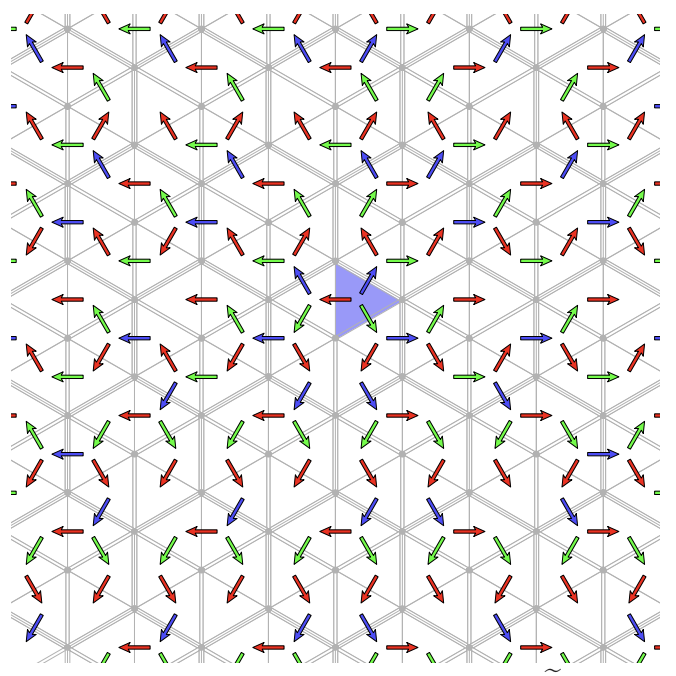
\includegraphics[width=0.4\linewidth]{Casselman_InverseShortLex.png}
    \caption{ShortLex words in $\widetilde{A}_2$, visualized as paths of reflections in the $\mathbb{R}^2$--tiling on which it acts}
    \label{fig:A2tilde}
\end{figure}

We trained a $256$D transformer, with a single $4$--head attention layer and an MLP layer of dimension $1024$
to learn {\em left} and {\em right} descent sets of length $\leq 36$ group elements in $\widetilde{A}_2$. Left (resp., right) descents of a Coxeter group element $g$ are the possible first (resp., last) letters of minimal-length words representing  $g$. Note that {\em minimal length} words in $\widetilde{A}_2$ are not unique, but their {\em ShortLex normal form} expressions are. The ShortLex normal form of a Coxeter group element is the unique minimal-length word that is lexicographically first with respect to a chosen ordering on the generators. 

We used three different data sets of increasing quality (unreduced, reduced, and ShortLex words representing elements of $\widetilde{A}_2$) in our experiments and found an accompanying clear improvement in model performance (Figures \ref{fig:RandomModelPerformance}, \ref{fig:ReducedModelPerformance}, and \ref{fig:ShortLexModelPerformance}) - test accuracy began deteriorating at length $5$ for the unreduced data set, at length $8$ for the reduced data set, and never for the ShortLex data set, which contained all ShortLex words of length 36. Our key takeaways are:


\begin{itemize}
    \item The attention patterns for the right descent task (Figure \ref{fig:RightDescents}) exhibit a same--parity structure, which motivated Proposition \ref{prop:OddIndicesDetermineLeftDescent}.
    \item The attention patterns for the left descent task (Figure \ref{fig:LeftDescents}) concentrate strongly on the beginning of the word, which motivated Proposition \ref{prop:6LetterEnough}.
    \item Quality and consistency of the data set was the most important factor determining model performance. Compare Figures \ref{fig:RandomModelPerformance} and \ref{fig:ReducedModelPerformance} with \ref{fig:ShortLexModelPerformance}.
 
%    \item Both train and test accuracy were nearly $100\%$ on the ShortLex benchmark for both descent tasks (Figures \ref{fig:LeftDescentAccuracy} and \ref{fig:RightDescentAccuracy}). 
\end{itemize}

\begin{figure}[h]
    \centering        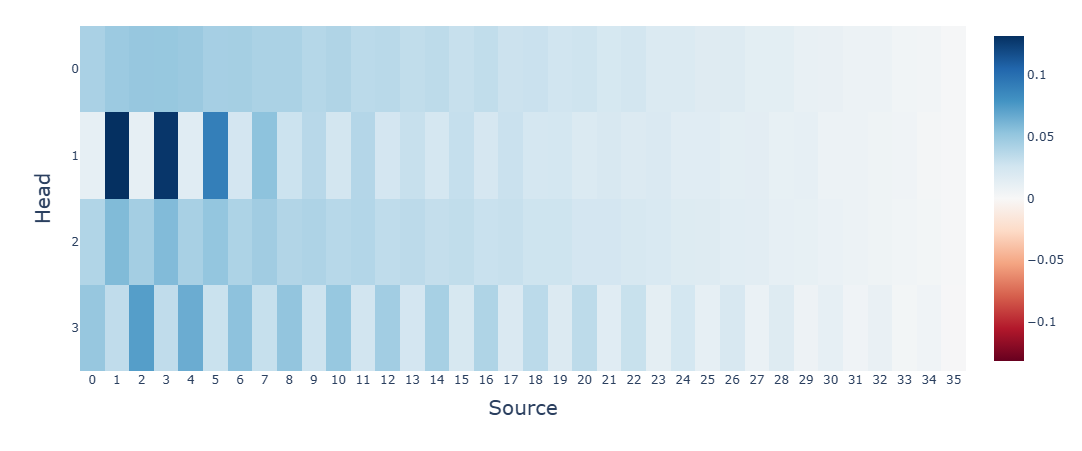
\includegraphics[width=0.6\linewidth]{A2_Short_lex_right.png}
    \caption{Right descent set prediction task: average attention paid by the final token in each of the $4$ attention heads, averaged over ShortLex normal form words of length $36$ in $\widetilde{A}_2$.} 
\label{fig:RightDescents}
\end{figure}  

\begin{figure}[h]
    \centering
    
        \centering    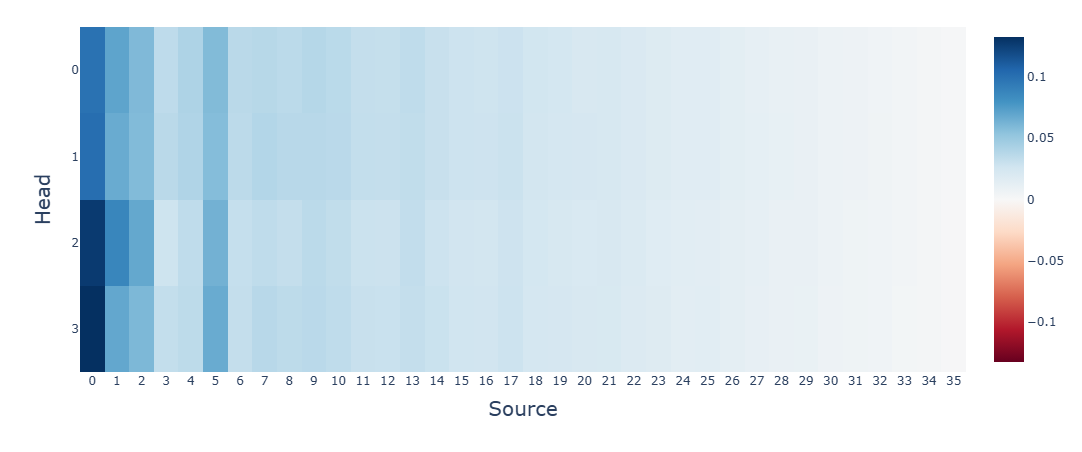
\includegraphics[width=0.6\linewidth]{A2_Short_Lex_left.png}
        \caption{Left descent prediction: Average attention of final token of length $36$ normal form word}
\label{fig:LeftDescents}
\end{figure}

  






\section{Related Work}
Mechanistic interpretability (cf. \citet{anthropic2022transformer, nanda2022comprehensive, Conmy, olsson2022induction}) is concerned with analyzing how the internal behavior of a model's parameters and latent features influences its outputs. Algorithmic tasks are a good fit, since a proposed circuit can be checked against a previously-known algorithm. The works that most directly influenced ours are \citet{nanda2022grokking}and \citet{Zhong}, which studied an (abelian) modular addition task and found evidence for Fourier-type circuits, and \citet{chughtai2023toy}, which studied a group multiplication task in some non-abelian finite groups, proposing a circuit implementing a representation-theoretic algorithm. In \citet{stander2024grokking}, the authors revisited the interpretation given in \citet{chughtai2023toy}, proposing an alternate interpretation in terms of quotient groups -- a reminder that even among experts, there is disagreement about what a model might have learned. %The pattern across this work is consistent. %Trained networks eventually appeared to land on clean, mathematically sensible solutions. 
In all of these works, the solution itself was well-known, and the mechanistic interpretability work provided evidence that the model learned the proposed algorithm.  Our work differs mainly in the complexity of the mathematical task. All of the works above explored a fixed operation on a {\em finite} group. We investigate an infinite group that enjoys a known finite word-processing algorithm \citet{Brink1993}. In our case, although an algorithm was known, the two results suggested by the model's solution - that we then proved without the aid of the model - do not follow immediately from the algorithm. We were inspired by \citet{LiuAshGoeelKrishZhang}, whose authors proposed a theoretical framework for understanding why transformer architectures might be particularly well-suited for learning elementary computational models called {\em finite state automata} or {\em finite state machines}. As far as we know, no prior mechanistic interpretability work has studied normal form expressions in infinite groups as a learning target. 

%\citet{stander2024grokking}  found that a transformer trained on modular addition learns a Fourier-based circuit. It places inputs on a circle by residue and adds them using trig identities.  showed this holds for arbitrary finite groups too. Networks learn an algorithm built on the group's irreducible representations. Weights, logits, and ablations all confirm it. But which specific circuit a network lands on, and in what order it develops, is largely arbitrary. 

%extended this to $S_5$ and $S_6$. Networks recover the true subgroup structure and compute products via cosets. They also found their account didn't fully match an earlier paper's explanation of the same setup 

%for look at descent sets instead --- a property of how a word is written, not an operation on two elements. And we work in Coxeter groups, an infinite family that includes affine and hyperbolic types with no finite-group equivalent. As far as we know, no prior mechanistic interpretability work has studied normal forms or descent sets as a learning target. We also found that learnability depends heavily on which normal form is used (cf. Section~\ref{sec:math-background} for the definition of normal form) --- something with no counterpart in the fixed-representation tasks above.

%A useful point of comparison is the broader landscape of domain-informed AI
%systems, which range from architectures that directly incorporate domain structure to architectures that leave the architecture general and shift interpretability elsewhere. \citet{Jumper2021} sits at one end of
%this spectrum: modules like Invariant Point Attention and triangle attention
%are built around the geometric structure of proteins, so that spatial
%reasoning is encouraged by the architecture itself rather than left for the
%model to discover. 

%\citet{merchant2023gnome} occupies a middle position,
%using graph neural networks that encode some relational structure from
%crystals (atoms as nodes, bonds as edges), though whether its internal
%computation reflects real chemical bonding logic remains an open question.
%\citet{bran2023chemcrow} represents a third strategy that sidesteps the
%problem entirely: the underlying LLM is unmodified, and all
%chemistry-specific reasoning happens outside the network, in a set of
%external tools it references.

%Our comparison across word representations echoes this same trade-off.
%Rather than building group structure into the architecture, we build it
%into the training data. We vary how structured that data is, from random
%words to the canonical ShortLex normal form. We then use attention analysis
%to check whether more structured training data produces more legible
%internal computation. This mirrors the role mechanistic interpretability
%plays for architectures like GNoME. GNoME's graph structure gives the model
%some chemical priors, like which atoms are bonded to which. But it does not
%guarantee the model's internal computation actually uses that structure the
%way a chemist would expect. The model's internals must be checked directly
%to know. In the same way, giving our model more structured training data
%does not guarantee it learns a cleaner internal representation of the
%group. Attention analysis is how we check whether it actually did.


%\citet{LiuMT23} investigate grokking and argue that it occurs when oversized starting weights cause a model to memorize small datasets first, while weight decay slowly shrinks the weights into an optimal size range.

%\citet{WangBY} show that Transformers can learn implicit knowledge-based reasoning through grokking, with the formation and configuration of generalizing circuits determining systematic generalization.

%\citet{Zhong} study neural networks trained on modular addition and show that small changes in architecture and hyperparameters can lead to qualitatively different solutions, including the "Clock" and "Pizza" algorithms.

%\citet{Zhou} find that pretrained LLMs solve addition by using low-frequency Fourier features in MLP layers to approximate the magnitude of the answer and high-frequency features in attention layers to compute its exact modular digits.

%\citet{stolfo} find that language models calculate arithmetic by using early layers to read the numbers, attention to transfer this information to the final token, and late MLP layers to generate the answer.

%\citet{Gould} identify "successor heads" in LLMs, a recurring type of attention head across different model sizes and architectures that performs incrementation using interpretable "mod-10" numeric features.

%\citet{Hanna} identify and analyze a circuit in GPT-2 Small that performs the greater-than operation, showing how its MLPs implement this mathematical ability across different contexts.

%\citet{WangJG} use Sparse Autoencoders to compare Transformer and Mamba models and find that they learn highly similar interpretable features and induction circuits, while also showing architecture-specific differences such as Mamba's "off-by-one" preference.

%\citet{Conmy} introduce Automatic Circuit DisCovery (ACDC), an algorithm that automates activation patching to identify functional computational subgraphs in Transformer models.

\section{Mathematical background}\label{sec:math-background}

We save a more detailed discussion of groups, group presentations, and general Coxeter groups for Appendix \ref{app:GroupsandCoxeter}. For now, suffice it to describe our main object of interest, the \textit{Coxeter group of type $\widetilde{A}_2$}:
\begin{equation}
\label{eq:A2tildepresentation}
\widetilde{A}_2 = \langle a_1, a_2, a_3 : a_i^2 \textup{ for all } i, \,\, (a_ia_j)^3 \textup{ for all } i\neq j\rangle.
\end{equation}
Elements of $\widetilde{A}_2$ can be represented by words (finite ordered strings) with letters in the set $S = \{a_1, a_2, a_3\}$ of {\em generators}. Moreover, two words $w,w'$ represent the same group element if $w'$ can be obtained from $w$ by finitely many insertions or deletions of the {\em relations}, which are the strings to the right of the colon in the {\em group presentation} for $\widetilde{A}_2$ given in  Equation \ref{eq:A2tildepresentation}.

Recalling that $\widetilde{A}_2$ can be understood as the symmetries of the tiling in Figure \ref{fig:A2tilde}, the relations $a_i^2$ arise because the generators are reflections, and the relations $(a_ia_j)^3$ (called {\em braid}  relations) arise because the product of two reflections across hyperplanes that intersect in an angle of $\theta$ produce a rotation of $2\theta$. Each group element $g$ can be represented by infinitely many different words; Let  $\ell(g)$ denote the length of a shortest word in the $a_i$ representing $g$. From this, we may define the \textit{left descent set} $D_L(g)$ and \textit{right descent set} $D_R(g)$ of $g$:
$$
D_L(g) = \{s\in S: \ell(sg) < \ell(g) \},
$$
$$
D_R(g) = \{s\in S: \ell(gs) < \ell(g) \}.
$$
% (we likewise define $\ell(w)$ for a word $w$ with letters in $S$ by setting it equal to the group element it defines.)
Given a word $w=s_1\ldots s_k$ with $s_i\in S$, we say it is of \textit{minimal length} if $\ell(w)=k$. We see that an element of $\widetilde{A}_n$ is not represented by a unique word of minimal length. For example, it follows from the relations that $a_1a_2a_1$ and $a_2a_1a_2$ are two minimal-length words representing the same group element in $\widetilde{A}_2$. To pick a distinguished minimal length representative, we pick the one that is first with respect to the lexicographic order $a_1 < a_2 < a_3.$ We say a word $w$ is in \textit{(ShortLex) normal form} if it is the unique word representing a group element that is first in lexicographic order. In the example above, $a_1a_2a_1 < a_2a_1a_2$, and therefore $a_1a_2a_1$ is the ShortLex normal form representative. In addition, we will say a word is \textit{reduced} if it contains no sub-word of the form $a_ia_i$ for any $i$.

\begin{figure}[h]
    \centering
    \begin{subfigure}{210 pt}
    \centering
    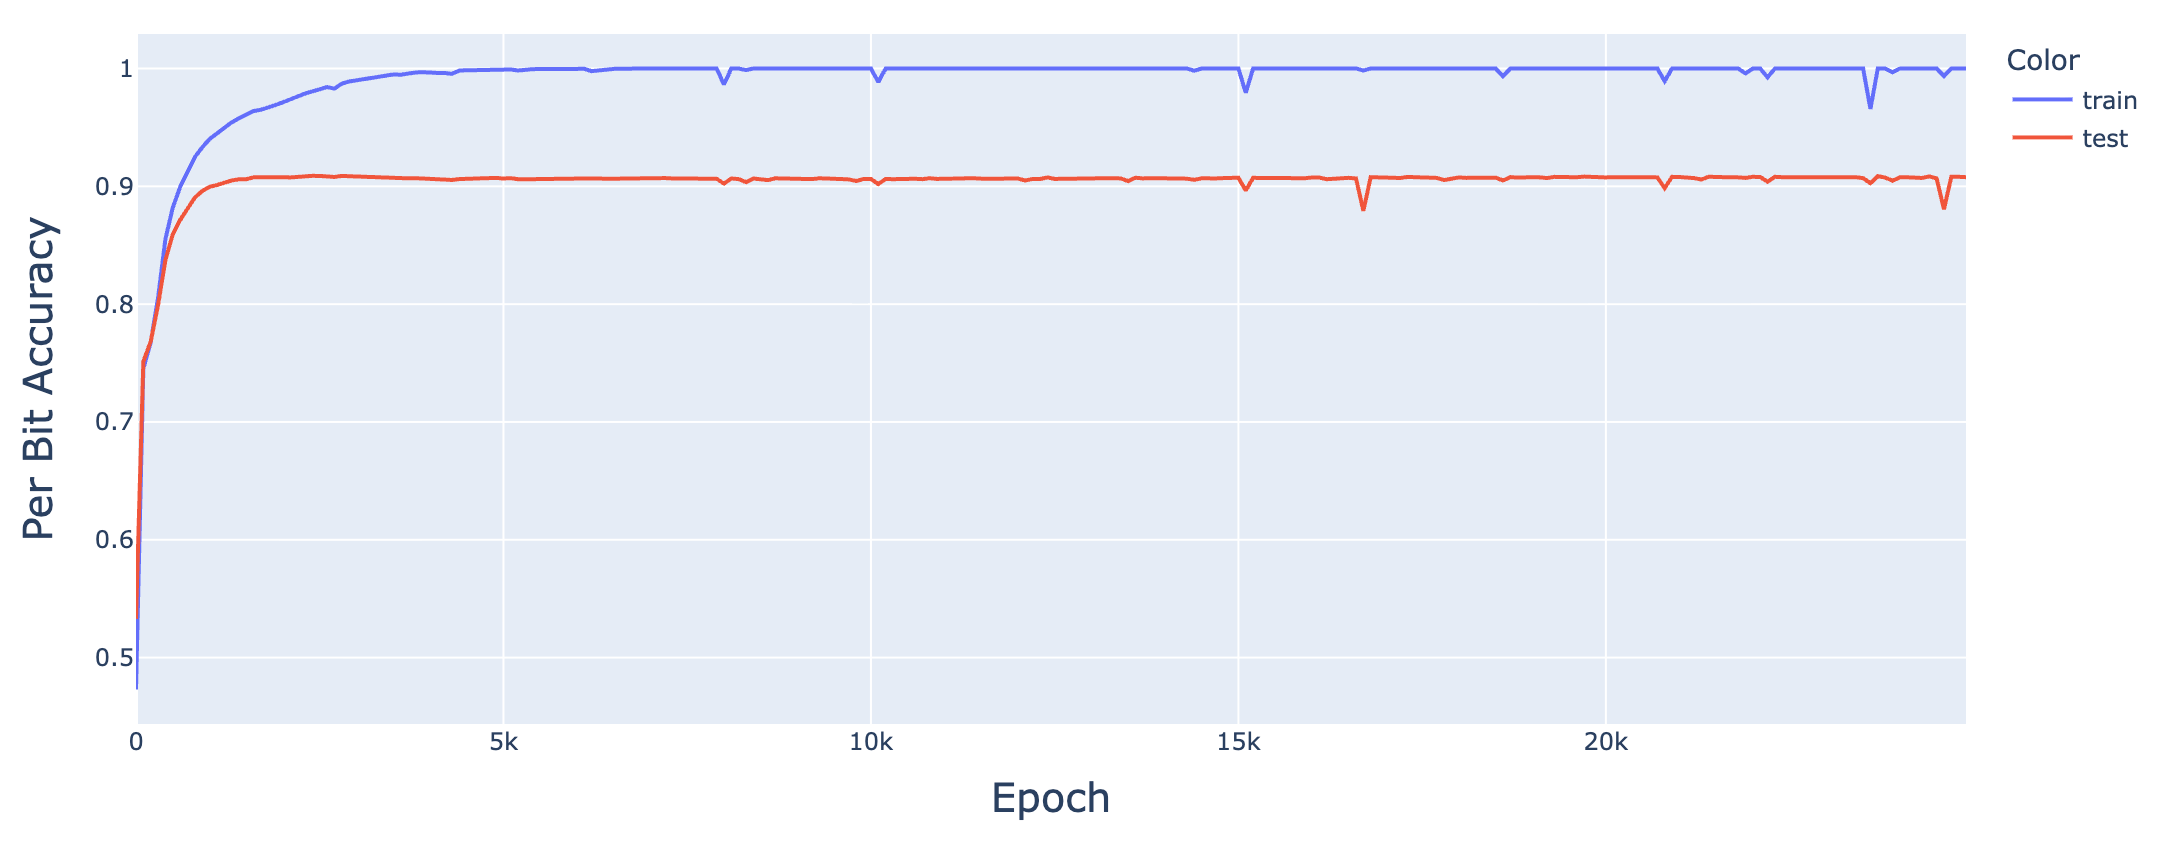
\includegraphics[width=\linewidth]{random_length_10_acc.png}
    \caption{Model accuracy for random words of length $10$}  \label{fig:RandomAccuracy10}    
    \end{subfigure} \hfill
    \begin{subfigure}{185 pt}
    \centering  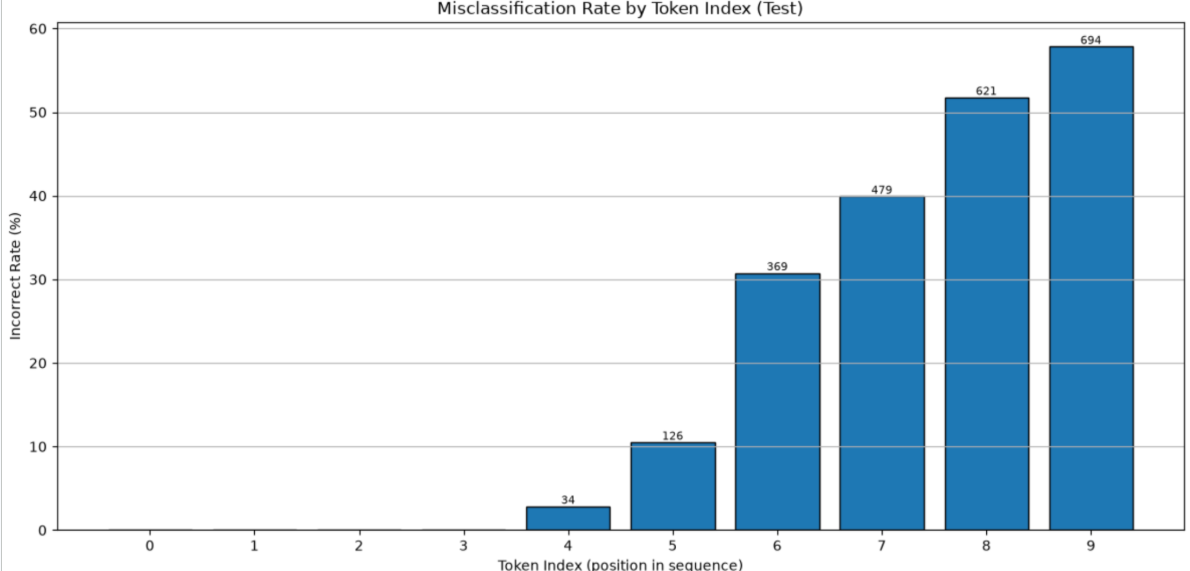
\includegraphics[width=\linewidth]{test_misclass_random.png}
    \caption{Misclassification by index for random words.}  \label{fig:RandomTestMisclass}
\end{subfigure}
\caption{Model performance for the left descent task on random words of length $10$ in $\widetilde{A}_2$.}
\label{fig:RandomModelPerformance}
\end{figure}


\begin{figure}[h]
    \centering
    \begin{subfigure}{210 pt}
    \centering
    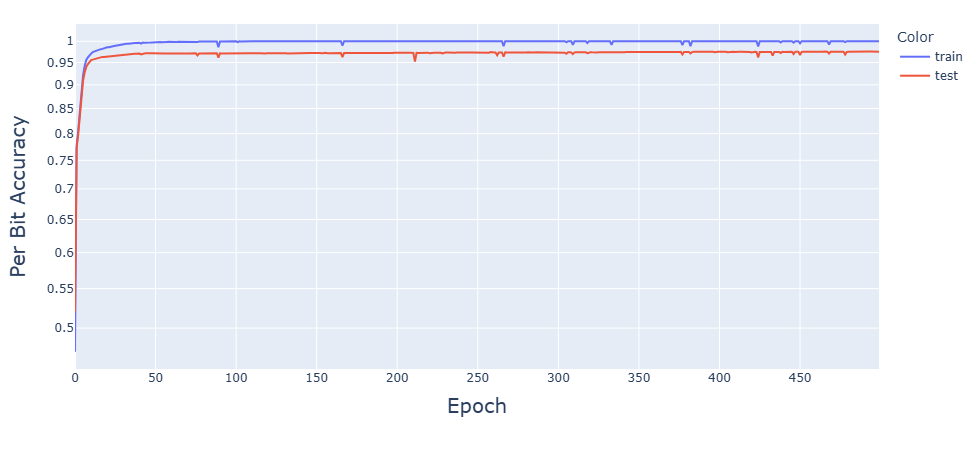
\includegraphics[width=\linewidth]{reduced_length_10_acc.png}
    \caption{Model accuracy for reduced  words of length $10$}  \label{fig:ReducedAccuracy10}    
    \end{subfigure} \hfill
    \begin{subfigure}{185 pt}
    \centering    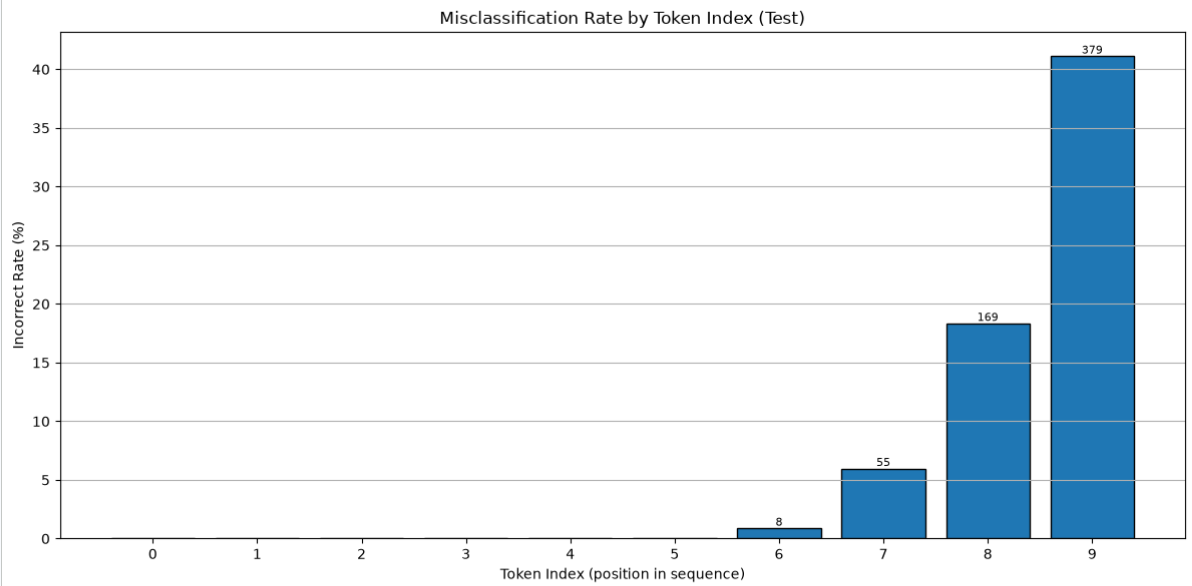
\includegraphics[width=\linewidth]{test_misclass_reduced.png}
    \caption{Misclassifications by index for reduced words.}  \label{fig:ReducedTestMisclass}
\end{subfigure}
\caption{Model performance for the left descent task on reduced words of length $10$ in $\widetilde{A}_2$}
\label{fig:ReducedModelPerformance}
\end{figure}

\begin{figure}[h]
    \centering
%    \begin{subfigure}{190 pt}
%    \centering
%    \includegraphics[width=\linewidth]{RightBitAcc_cropped.png}
%    \caption{Model accuracy for right descent of words in $\widetilde{A}_2$.}  \label{fig:RightDescentAccuracy}    
%    \end{subfigure} \hfill
    \begin{subfigure}{195 pt}
    \centering    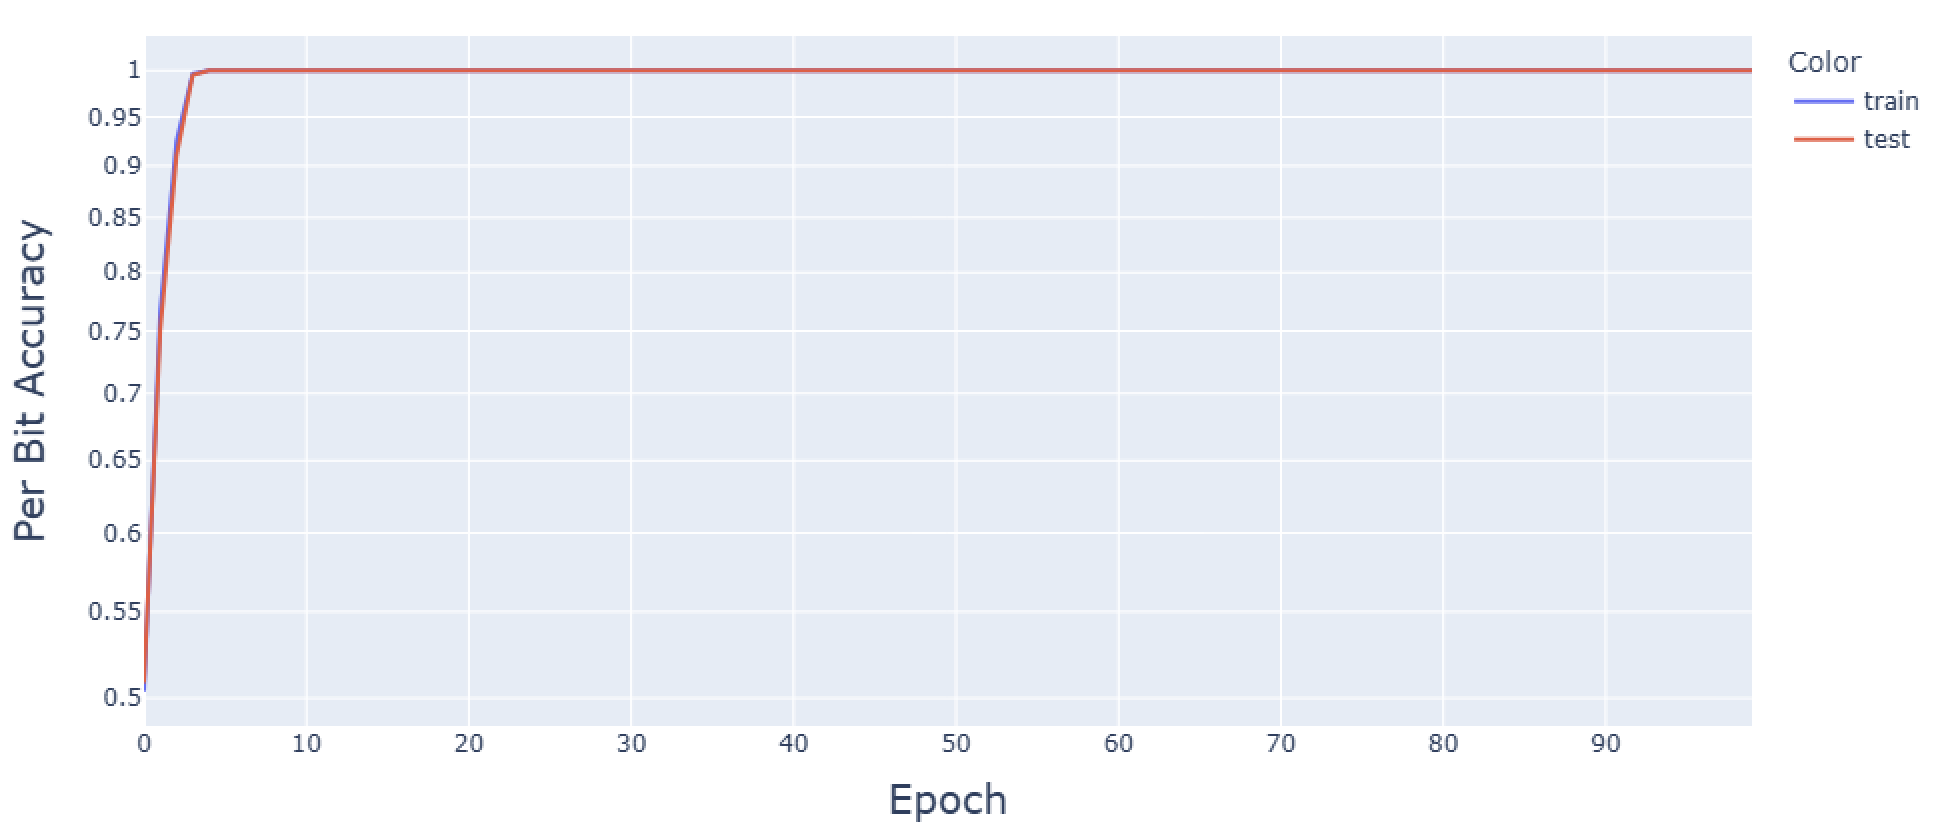
\includegraphics[width=\linewidth]{LeftBitAcc_cropped.png}
    \caption{Model accuracy for ShortLex words of length $\leq 36$}  \label{fig:LeftDescentAccuracy}
\end{subfigure}
    \begin{subfigure}{195 pt}
    \centering    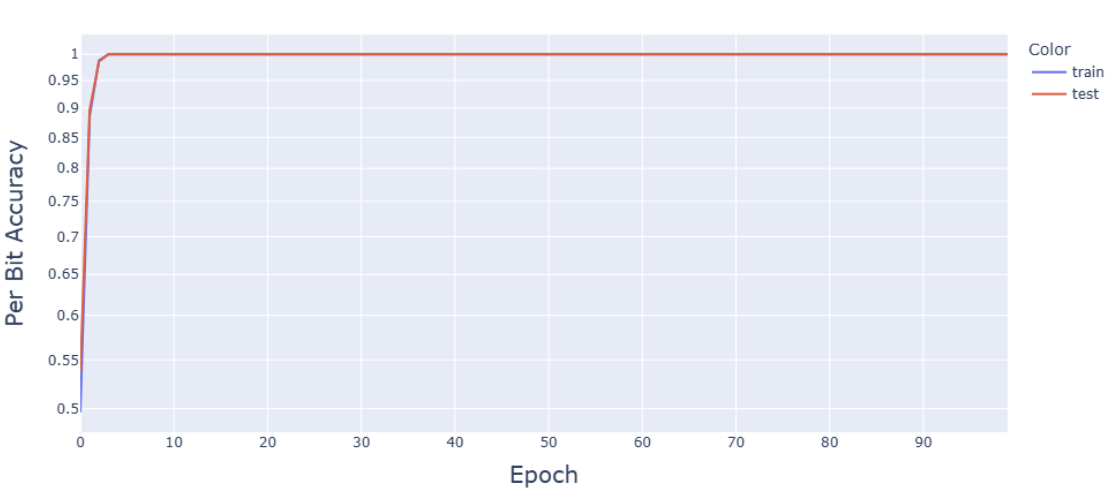
\includegraphics[width=\linewidth]{MaskAfterFirst5.png}
    \caption{Model accuracy when all but first $5$ tokens masked}  \label{fig:AllButFirst5MaskedAccuracy}
\end{subfigure}
\caption{Model accuracy for the left descent task on ShortLex words in $\widetilde{A}_2$ of length up to $36$. The model achieved nearly $100 \%$ test accuracy (left), and performance remained strong (right) when all but the first $5$ tokens were masked, supporting Proposition \ref{prop:6LetterEnough}.}% a subset of input tokens is masked during training. Test and train accuracy were nearly $100\%$ on the left descent task when no tokens were masked, stayed at nearly $100\%$ when all but the first $5$ tokens were masked, and dropped to below $70\%$ on the test set when the first $5$ tokens were masked.}
\label{fig:ShortLexModelPerformance}
\end{figure}


We formulated and proved the following two results after observing the attention patterns (Figures \ref{fig:RightDescents} and \ref{fig:LeftDescents}) in the transformer model trained on the ShortLex data set. The statements are likely to be known by experts, but we never found explicit references to them in the literature. Their proofs are in Appendix \ref{app:GroupsandCoxeter}.

\begin{proposition}[Odd-indices determine right descent]\label{prop:OddIndicesDetermineLeftDescent}
Let $w$ be a length $n \geq 2$ word which is minimal length for an element of  $\widetilde{A}_2$. The right descent set of $w$  is a subset of the final two letters of $w$, contains the final letter of $w$, and
contains the penultimate letter of $w$ iff $w$ contains a braid-flippable pattern at an index $i$ with $i \equiv n \mod 2$. I.e., there is some $ i \equiv n \mod 2$ with $s_i = s_{i+2}$.
\end{proposition}

\begin{proposition}[Bounded initial string determines left descent]\label{prop:6LetterEnough}
The left descent set of any element of $\widetilde{A}_2$ is completely determined by the first six letters of its ShortLex normal form representative.
\end{proposition}

\section{Experimental setup and results}

We created three different increasingly structured $\widetilde{A}_2$ data sets for training: random words, reduced words, and ShortLex normal form words. For the random-word experiment, we generated 2,000 words of length 10 at random from $S = \{a_1, a_2, a_3\}$, allowing repetition of adjacent generators. The reduced-word dataset similarly contained 2,000 words of length 10, but adjacent generators were required to be different. For both datasets, we used a $40/60$ train/test split. Because there are substantially fewer ShortLex normal form words of any given fixed length, and we wanted to ensure that no complete test words appeared in the training set, we used all 1,998 ShortLex normal-form words of length at most 36, with a 30/70 train--test split. %Together, these three datasets allow us to test whether increasingly structured, higher-quality representations make the underlying group structure easier for the transformer to learn.
Words were labeled by either their left or right descents at each prefix. Labels were binary $3$--tuples, with a $1$ indicating membership of the corresponding generator in the descent set. For example, the label $(1,0,1)$ at position $1\leq k \leq n$ in a word $w = s_1 \cdots s_k \cdots s_n$ would indicate that there exist minimal length words representing the group element $s_1 \cdots s_k$ ending in $a_1$ and $a_3$, but not $a_2$.

Across all experiments, we built atop the \textbf{TransformerLens} \citep{nanda2022transformerlens} package, an open-source library for mechanistic interpretability of GPT-2-style models. For all experiments we used a $256$--dimensional model with a single attention layer with $4$ heads and a hidden MLP layer of dimension $1024$. 
The output layer was dimension $3$ with logistic sigmoid activation on each output neuron to predict membership in the descent set. The model was trained autoregressively with component-wise binary cross entropy loss, with a weight decay of $0.5$.

In the ShortLex experiments, the model generalized very well to data it hadn't seen. Of all test subwords from our ShortLex dataset on the left descent task, $2\%$ were unseen during training, and all were of length $>26$. The model achieved $100 \%$ accuracy on them. A second run with a  $90/10$ train test split achieved $99.3 \%$ accuracy on unseen subwords, with $12.4 \%$ ($5462$ subwords) unseen during training. Finally, on a manually split dataset consisting of all 63 words of length $\leq 6$ along with $136$ random longer words, $16.3 \%$ of the test subwords (7,335 subwords) were unseen, and the model achieved $100 \%$ accuracy on the unseen data.



%Our experiments were designed to study two questions: how the choice of word representation affects the transformer's ability to learn descent sets, and what the model's attention patterns reveal about the structure of left descent sets in $\widetilde{A}_2$.




%For the experiments, words were labeled by their left or right descent sets. The model predicts the corresponding descent set at each prefix of the input word. We train separate models for left and right descent prediction.


%In addition to predictive accuracy, we examine the attention patterns learned by the ShortLex descent-set models. In the left-descent experiment, the learned attention concentrates on the first six letters of the word, suggesting that this initial segment may be sufficient to determine the left descent set. For comparison, in the right-descent experiment, the attention head looks back across the entire word, alternating between positions.



\section{Conclusions and future work}

Our experiments show that a small transformer can achieve high accuracy on combinatorial word-theoretic tasks in the infinite Coxeter group $\widetilde{A}_2$, and that its learned attention patterns can suggest mathematical structure. It would be interesting to apply these methods to other families of infinite Coxeter groups and to use more advanced mechanistic interpretability tools to extract and validate circuits implementing the known Brink-Howlett finite state automata \citet{Brink1993} for these groups. Note that implicit within the Brink-Howlett FSA is an algorithm to determine descent sets. It would be interesting to explicitly see this algorithm as computational circuits in the model.

\section{Generative AI statement} Generative AI helped with coding, figures, and literature search, but not with proofs or prose.
%\begin{figure}
%    \centering
%    \includegraphics[width=0.5\linewidth]{3. Hyper_Short_lex_Left.png}
%    \caption{Attention pattern for left descents of words in the [4,3,3] hyperbolic group.}
%\end{figure}


%\begin{figure}
%    \centering
%    \includegraphics[width=0.5\linewidth]{3. Hyperbolic Left Bit Acc.png}
%    \caption{Model accuracy for left descent of words in the [4,3,3] hyperbolic group.}
%\end{figure}



\appendix
\section{Group presentations and Coxeter groups}\label{app:GroupsandCoxeter}

The following background in group theory and the theory of Coxeter groups is standard. See for example \citet{artin2011algebra} and \citet{BjornerBrentiCoxeter}.

\subsection{Groups} 

A {\em group} $G$ is a set equipped with a binary operation \[\cdot: G \times G \rightarrow G\] called {\em multiplication} that satisfies the following properties:
\begin{enumerate}
        \item \emph{Associativity:} For all $a,b,c\in G$, $(a\cdot b)\cdot c=a\cdot(b\cdot c)$.
        \item \emph{Identity:} There exists an element $e\in G$, called the \emph{identity element}, such that $a\cdot e=e\cdot a=a$ for all $a\in G$.
        \item \emph{Inverses:} For every $a\in G$, there exists an element $a^{-1}\in G$, called the \emph{inverse} of $a$, such that $a\cdot a^{-1}=a^{-1}\cdot a=e.$
\end{enumerate}
A \emph{finite presentation} $G=\langle S\mid R\rangle$ of a group $G$ consists of: 
\begin{enumerate} 
\item A finite set $S$, whose elements are called the \emph{generators} of the presentation. 
\item A finite set $R$ of elements of the form $s_1^{n_1}\ldots s_l^{n_l}, n_l\in \mathbb{Z}, s_i\in S$, representing the identity element of $G$. Such elements are called the \emph{relations} of the presentation. 
\end{enumerate}
We assert that two words $w,w'$ represent the same group element if $w'$ can be obtained from $w$ by finitely many insertions or deletions of the relations.
\subsection{Coxeter groups} 

Let $S$ be an indexed finite set. A {\em Coxeter matrix} is a matrix given by the function,
\[
    m:S \times S \longrightarrow \mathbb{N} \cup \{\infty\}
\]
which satisfies
\begin{enumerate}
    \item $m(s,s') = m(s',s)  \textup{ for all } s,s' \in S$,
    \item $m(s,s') = 1 \text{ if and only if } s=s'$.
\end{enumerate}

The {\em Coxeter group} $W_m$ associated to Coxeter matrix $m$ is given by
$$
W_m = \langle S \mid (s_i s_j)^{m(s_i,s_j)}=e : s_i,s_j \in S \rangle.
$$
Here, the relations of the form $(s_i s_j)^{m(s_i,s_j)}=e$ for $i\neq j$ are called the \textit{braid relations}. On the other hand, since $m(s,s)=1$, every generator satisfies $s^2=e.$ Thus, two adjacent copies of the same generator in a given word may be removed without changing the represented group element.

\subsection{(Un)reduced words, minimal length words, and normal form} 
\label{sec:reduced-unreduced-words}
A \emph{word} with letters in $S$ is a finite sequence \[ w=s_1s_2\cdots s_k, s_i\in S. \] Its word length is the number of generators it contains: $|w|=k.$ In this paper, a word is called \emph{reduced} if it contains no two identical generators next to each other. Equivalently, $ s_i\neq s_{i+1} \text{ for all }1\leq i<k.$ 
A word is called \emph{unreduced} if it contains an adjacent repeated pair $ss$. 

A group element in a Coxeter group may be represented by many different words. The \emph{length} of an element $w\in W_m$, denoted $\ell(w)$ is given by \[ \ell(w) = \min \left\{ k: s'_1\cdots s'_k, s'_i\in S, w = s'_1\cdots s'_k \textup{ in } W_m \right\}. \] Likewise, we shall say a given representation $s_1\ldots s_k$ of $w$ is of \textit{minimal length} if $k=\ell(w)$. In general, such a minimal length representation is not unique, and so fixing an ordering $s_{i}<s_{i+1}$, we get reverse-lexicographically get a unique representative of $w$ among its minimal length representations, called the \textit{Reverse ShortLex normal form}. Alternatively, we shall call the unique expression of minimal lexicographic order the \textit{ShortLex normal form}.
\subsection{Descent sets} 
\label{sec:descent-sets}
Let $w\in W_m$. The \emph{right descent set} of $w$ is 
\[ 
D_R(w) = \left\{ s\in S: \ell(ws)<\ell(w) \right\}. 
\] 
%Here, $\ell(w)$ denotes the minimum length of any word representing $w$. Thus, a generator $s$ belongs to $D_R(w)$ if multiplying $w$ by $s$ on the right produces an element whose shortest representation is shorter than that of $w$.

Similarly, the \emph{left descent set} of $w$ is 
\[ 
D_L(w) = \left\{ s\in S: \ell(sw)<\ell(w) \right\}. 
\]
%A generator $s$ belongs to $D_L(w)$ if multiplying $w$ by $s$ on the left decreases its Coxeter length.

For every generator $s\in S$, multiplication by $s$ changes Coxeter length by exactly one: 
\[ 
\ell(ws)\in\{\ell(w)-1,\ell(w)+1\}, 
\]
and similarly, 
\[ 
\ell(sw)\in\{\ell(w)-1,\ell(w)+1\}. 
\] 
Likewise, $s\in D_R(w)$ if and only if some minimal length expression for $w$ ends in $s$, and $s\in D_L(w)$ if and only if some minimal length expression for $w$ begins with $s$.

\section{The Coxeter group $\widetilde{A}_2$}
\par %\citet{Brink1993} proved that every finitely generated Coxeter group is automatic. That is, for a given Coxeter system $(W, S)$, there exists a regular language of word representatives for the group elements, alongside finite-state automata that verify right-multiplication by generator elements in quadratic time. By constructing a deterministic finite automaton based on the finite set of elementary roots, their framework establishes that the set of reduced expressions, as well as its sublanguage of ShortLex normal forms obtained by pruning non-minimal transitions, forms a regular language. Consequently, this construction applies directly to the affine Coxeter group $\widetilde{A}_2$, guaranteeing an explicit regular language of canonical word representatives recognized by a finite-state automaton.
\par Here, we prove Propositions \ref{prop:OddIndicesDetermineLeftDescent} and \ref{prop:6LetterEnough} through the proofs of Propositions \ref{prop:OddIndicesDetermineLeftDescentPrecise} and \ref{prop:6LetterEnoughPrecise}. We first see that Proposition \ref{prop:OddIndicesDetermineLeftDescent} is equivalent to:
\begin{proposition}\label{prop:OddIndicesDetermineLeftDescentPrecise}
    Let $w=s_1\ldots s_k$ be a word with letters $a_1, a_2, a_3$ of minimal length in $\widetilde{A}_2$. Then the left descent set of $w$ is $\{s_1, s_2\}$ if and only if there exists an odd index $i$ such that $s_i = s_{i+2}$. Otherwise $D_L(w)=\{s_1\}$.
\end{proposition}
This equivalence derives from the general Coxeter group fact that $D_L(w)=D_R(w^{-1})$, where $w^{-1}=s_k\ldots s_1$ for $w=s_1\ldots s_k$. Then, using this proposition, we prove Proposition \ref{prop:6LetterEnoughPrecise}, which implies Proposition \ref{prop:6LetterEnough}. The proofs also make use of algorithm detailed in \cite[Pseudocode, p. 13]{casselman2008computationcoxetergroupsii} for the left-multiplication of words in normal form by a generator. Foregoing a detailed discussion of the algorithm, we shall state here the minimal root look up table\cite[p.8]{casselman2008computationcoxetergroupsii} of $\widetilde{A}_2$:
\begin{center}
    \begin{tabular}{|c|c|c|c|}
        \hline
         & $a_1$ & $a_2$ & $a_3$ \\
        \hline
        $\alpha_{a_1}$ & $\ominus$ & $\alpha_4$ & $\alpha_6$ \\
        \hline
        $\alpha_{a_2}$ & $\alpha_4$ &$\ominus$ & $\alpha_5$\\
        \hline
        $\alpha_{a_3}$ & $\alpha_6$ & $\alpha_5$ &$\ominus$ \\
        \hline
        $\alpha_4$ & $\alpha_{a_2}$ & $\alpha_{a_1}$ & $\oplus$ \\
        \hline
        $\alpha_5$ & $\oplus$ & $\alpha_{a_3}$ & $\alpha_{a_2}$\\
        \hline
        $\alpha_6$ & $\alpha_{a_3}$ &$\oplus$ & $\alpha_{a_1}$\\
        \hline
    \end{tabular}
\end{center}
This table allows us to compute a certain value, $s\alpha$, where $s$ comes from one of the elements of the top row and $\alpha$ comes from one of the elements of the first column, which is an essential computation in the multipliation algorithm.\footnote{Explicitly, this computes the Weyl group action of the generators of $\widetilde{A}_2$ on its \textit{minimal roots}\cite[p. 7]{casselman2008computationcoxetergroupsii}. The notation $\ominus$ denotes the action of $s$ onto $\alpha_s$, and the notation $\oplus$ denotes $s\alpha$ producing a non-minimal positive root. That these are recorded in place of the roots is to provide sufficient conditions for the algorithm to end. In a particular, one understands that $\ell(sw)=\ell(w)-1$ if and only if $\ominus$ occurs somewhere in the root look up computation.}  Finally, throughout this section, for the sake of clarity and to prevent abuse of notation, we shall use $=$ to indicate equality on the level of words and $\sim$ to indicate equality on the level of group elements in $\widetilde{A}_2$. 

\begin{comment}
    

\begin{lemma}\label{lem:PossibleDescents}
    Let $w$ be a word of minimal length starting with $s_1s_2$. Then the left descent set is a subset of $\{s_1, s_2\}$ and contains $s_1$. 
\end{lemma}
\begin{proof}
    The problem being symmetric with respect to the choice of $s_1,s_2$ we shall assume without loss of generality that $s_1=a_3$ and $s_2=a_2$. There must exist an ordering of $a_1, a_2, a_3$ such that its Inverse ShortLex normal form must begin with $a_3a_2$, and so we may assume $w$ is in Inverse ShortLex normal form. Then by the algorithm presented in \citet[Pseudocode, p.13]{casselman2008computationcoxetergroupsii}, we see that $NF(a_1w)=a_1w$. This means that $a_1$ is not a left descent of $w$, as desired.
\end{proof}
\end{comment}

\begin{lemma}\label{lem:2Weyl1Root}
    Let $s_1, s_2, s_3$ be mutually distinct generators, and let $\alpha_{s}$ be as in \citet[p. 3]{casselman2008computationcoxetergroupsii} (that is the standard realization.) Then $s_2s_1\alpha_{s_2} = \alpha_{s_1}$
\end{lemma}
\begin{lemma}\label{lem:aba5LetterCase}
    Let $w = s_1\ldots s_5$ be a word with letters $a_1, a_2, a_3$ of minimal length in $\widetilde{A}_2$. If $s_3=s_5$ and $s_1 \neq s_3$ then $w\sim s_1s_2s_1s_3s_1$.
\end{lemma}
\begin{proof}
    As $s_1\neq s_3$, we see that $s_2$ must be distinct to $s_1$ and $s_4$. likewise $s_4=s_1$ since it cannot be $s_3$ and $s_2$: $s_3s_3\sim \textup{[empty]}$ and $s_2s_3s_2s_3 \sim s_3s_2$, which by the minimal length of $w$ implies that $w=s_1s_2s_3s_1s_3$. Then using the braid relation $s_1s_3s_1\sim s_3s_1s_3$, we get that $w\sim s_1s_2s_1s_3s_1$, as desired.
\end{proof}
\begin{lemma}\label{lem:abaGeneralCase}
    Let $w = s_1\ldots s_k$ be a minimal length word in the generators $a_1, a_2, a_3$ of  $\widetilde{A}_2$. If $s_i = s_{i+2}$ for some odd index $i$, then there exists a representation of $w$ starting with $s_1s_2s_1$. 
\end{lemma}
\begin{proof}
    If $s_1\ldots s_k$ is of minimal length, then $s_1\ldots s_l$ is of minimal length for all $l\leq k$. So the proof of this reduces to the case where $s_i=s_{i+2}$ if and only if $i=k-2$. In this case, we may proceed via recursion by Lemma \ref{lem:aba5LetterCase}, completing the proof. 
\end{proof}
\begin{proof}[Proof of Proposition \ref{prop:OddIndicesDetermineLeftDescentPrecise}]
    The if part of the proof follows from the lemmas above, and a direct calculation. Now to show the only if part, we see that there are two remaining cases to consider: $w=s_1\ldots s_k$ such that
    \begin{itemize}
        \item there is an even index $s_i = s_{i+2}$ but no odd index,
        \item there are no indices such that $s_i=s_{i+2}$.
    \end{itemize}
    \par Let us start by assuming that there is an even index $s_i = s_{i+2}$ but no such odd index. Then by an analogous argument to the one used in Lemma \ref{lem:abaGeneralCase}, there exists two minimal length representatives of $s_1\ldots s_k$ starting with $s_1s_2s_3s_2$ and $s_1s_3s_2s_3$ respectively. Now we recall (cf. \citet{casselman2008computationcoxetergroupsii}) that $D_L(w) = D_R(w^{-1})$ and that $s$ is a right descent of $w$ iff $w^{-1}$ applied to its associated simple root $\alpha_s$ evaluates negatively on the fundamental alcove (the purple triangle in Figure \ref{fig:A2tilde}). 
    
    We now consider the cases $\ell(w) := k=4$, and $k > 4$ separately. If $k=4$, we note first that by symmetry we may assume that $s_1 = a_1, s_2 = a_2, s_3 = a_3$. Then it is immediate from Figure \ref{fig:evenindexending} that $D_R(w^{-1}) = D_L(w) = \{s_1\}$, since its associated simple root $\alpha_{s_1}$ is the only one of the three that is negative on the fundamental alcove in the figure. If $k > 4$, then it is immediate from the fact that $D_R(s_1s_2s_3s_2) = \{s_2,s_3\}$ that $w \sim s_1s_2s_3s_2s_1w_0$ for some minimal length (possibly empty) word $w_0$. In this case, we need to argue that regardless of what $w_0$ is, $w^{-1} = (w_0)^{-1}(s_1s_2s_3s_2s_1)$ applied to $\alpha_{s_2}$ and $\alpha_{s_3}$ are both positive on the fundamental alcove, and hence neither $s_2$ nor $s_3$ is in $D_R(w^{-1}) = D_L(w)$. This can be seen by noting that since $s_1 \neq s_2 \neq s_3$, the action of $s_1s_2s_3s_2s_1$ on any alcove is to reflect it (and its markings by simple roots) across a hyperplane dominating $w_0^{-1}\alpha_{s_1}$, in the language of \citet{casselman2008computationcoxetergroupsii}. The conclusion follows from the observation that such a reflection will always send $w_0^{-1}(\alpha_{s_2})$ and $w_0^{-1}(\alpha_{s_3})$ to positive roots. See Figure \ref{fig:Dominatingreflection}.

    \begin{figure}
        \centering
        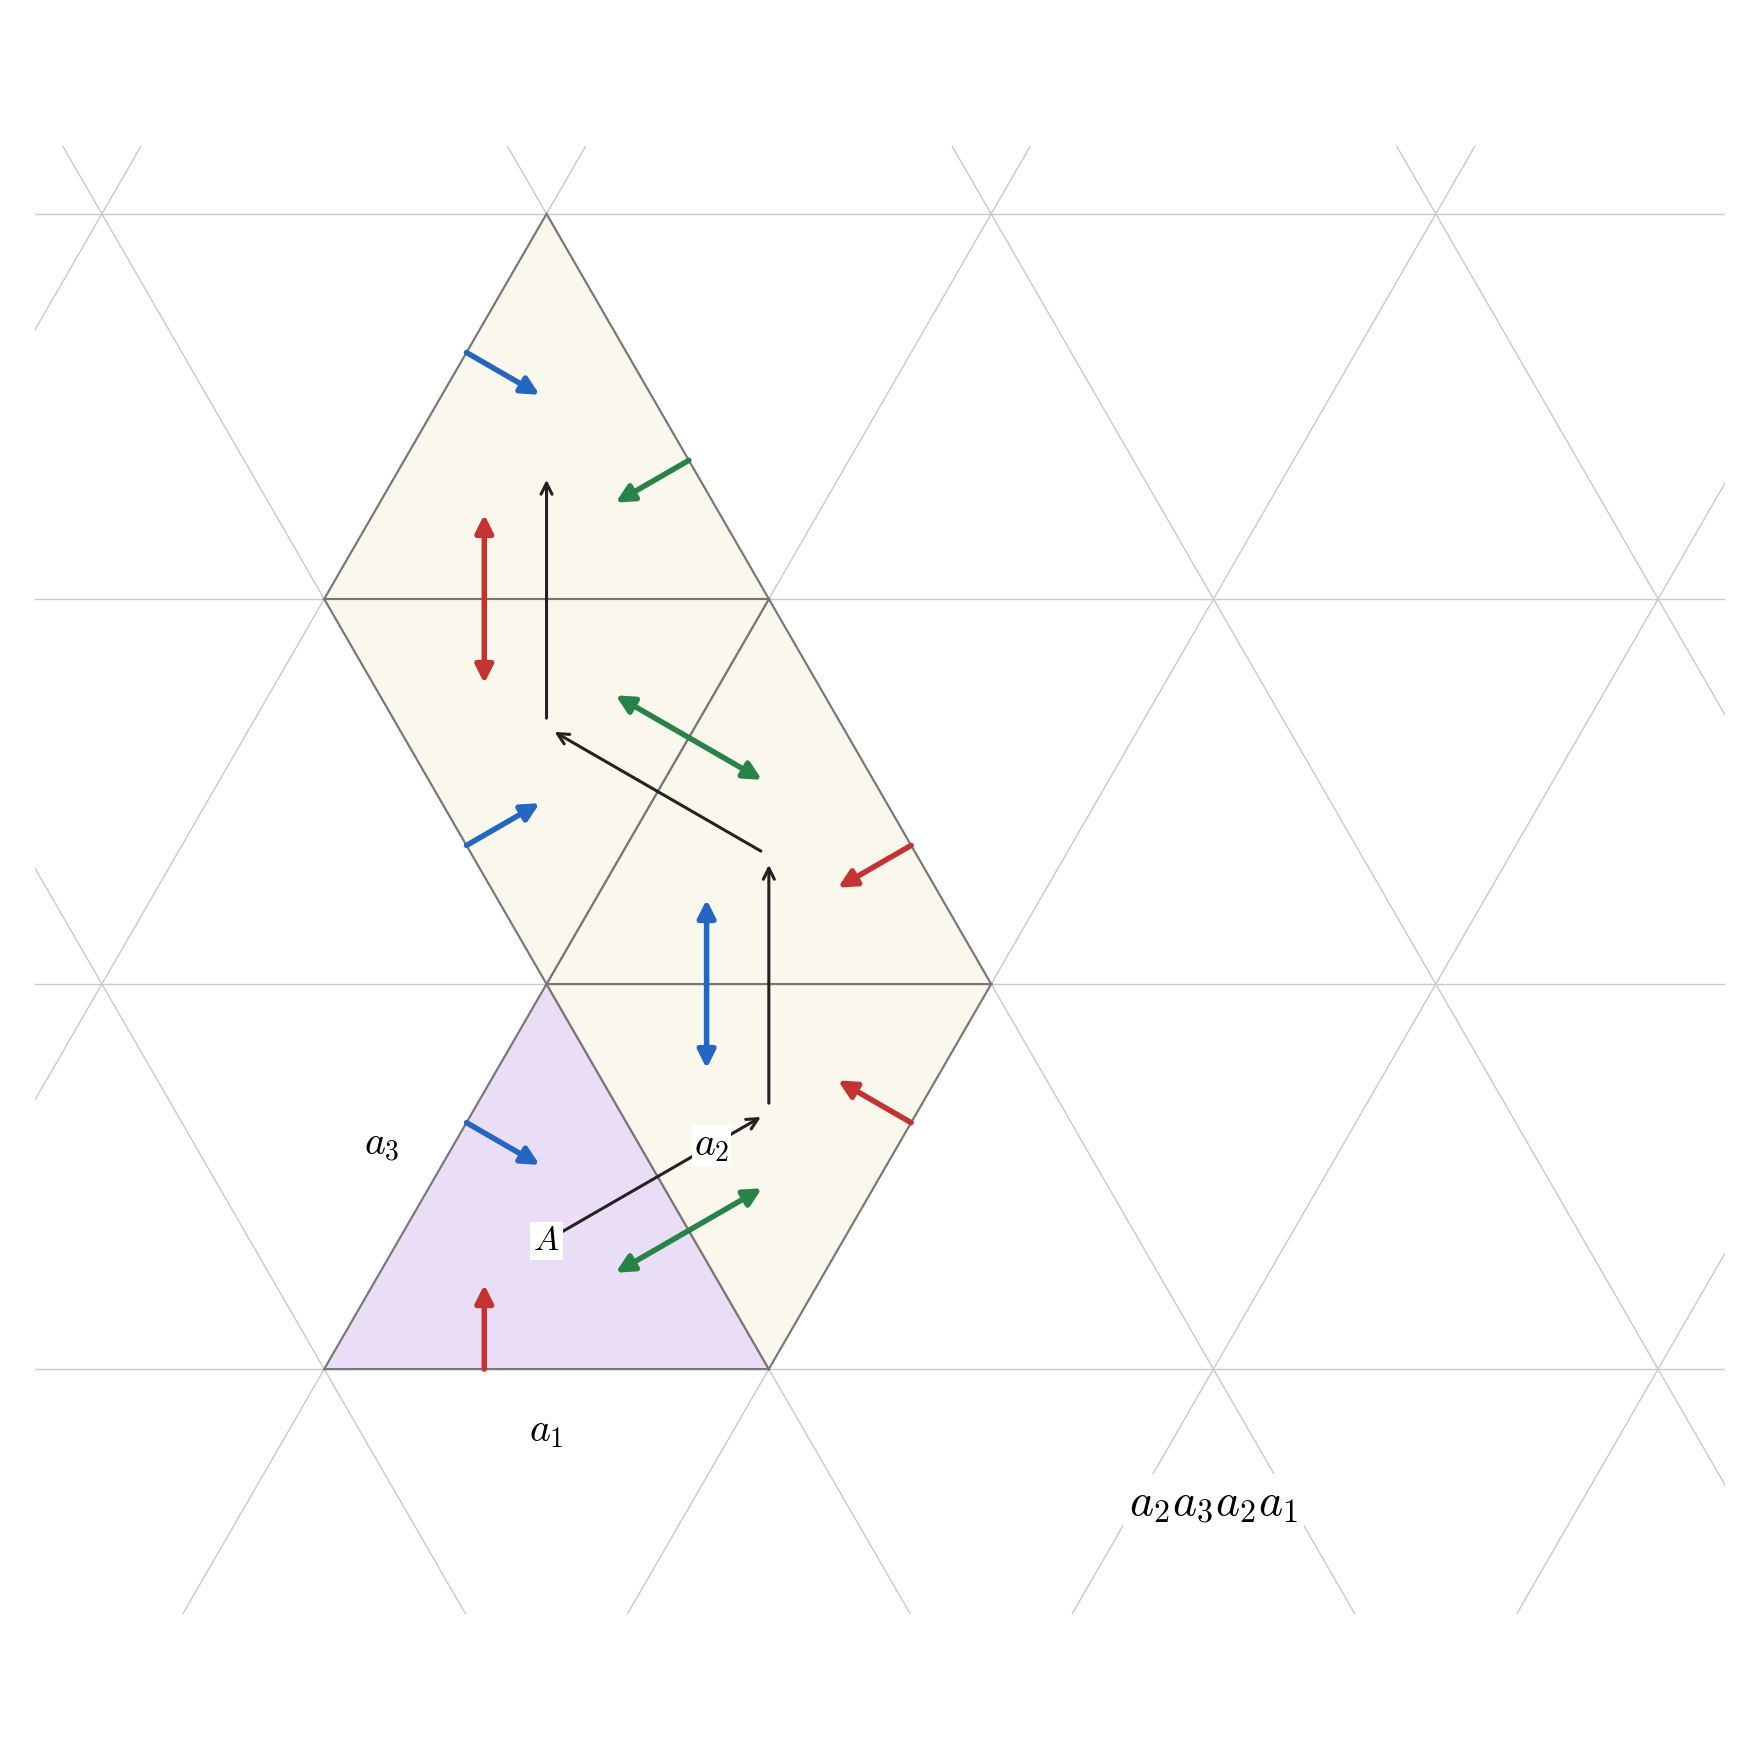
\includegraphics[width=0.60\linewidth]{affine_a2_path_2321_roots.png}
        \caption{The gallery associated to $w^{-1} = a_2a_3a_2a_1$ for $w = a_1a_2a_3a_2$, with fundamental alcove $A$ (associated to the identity element of $\widetilde{A}_2$) marked in purple, and simple roots $\alpha_{a_1}, \alpha_{a_2}, \alpha_{a_3}$ marked in red, green, blue, respectively. Note that at the endpoint of the gallery, $w^{-1}(\alpha_{a_1})$ is negative, confirming that $a_1 \in D_L(w)$, and $w^{-1}(\alpha_{a_2}), w^{-1}(\alpha_{a_3}) $ are positive, confirming that $a_2,a_3 \not\in D_L(w)$.}
        \label{fig:evenindexending}
    \end{figure}

    \begin{figure}
        \centering
        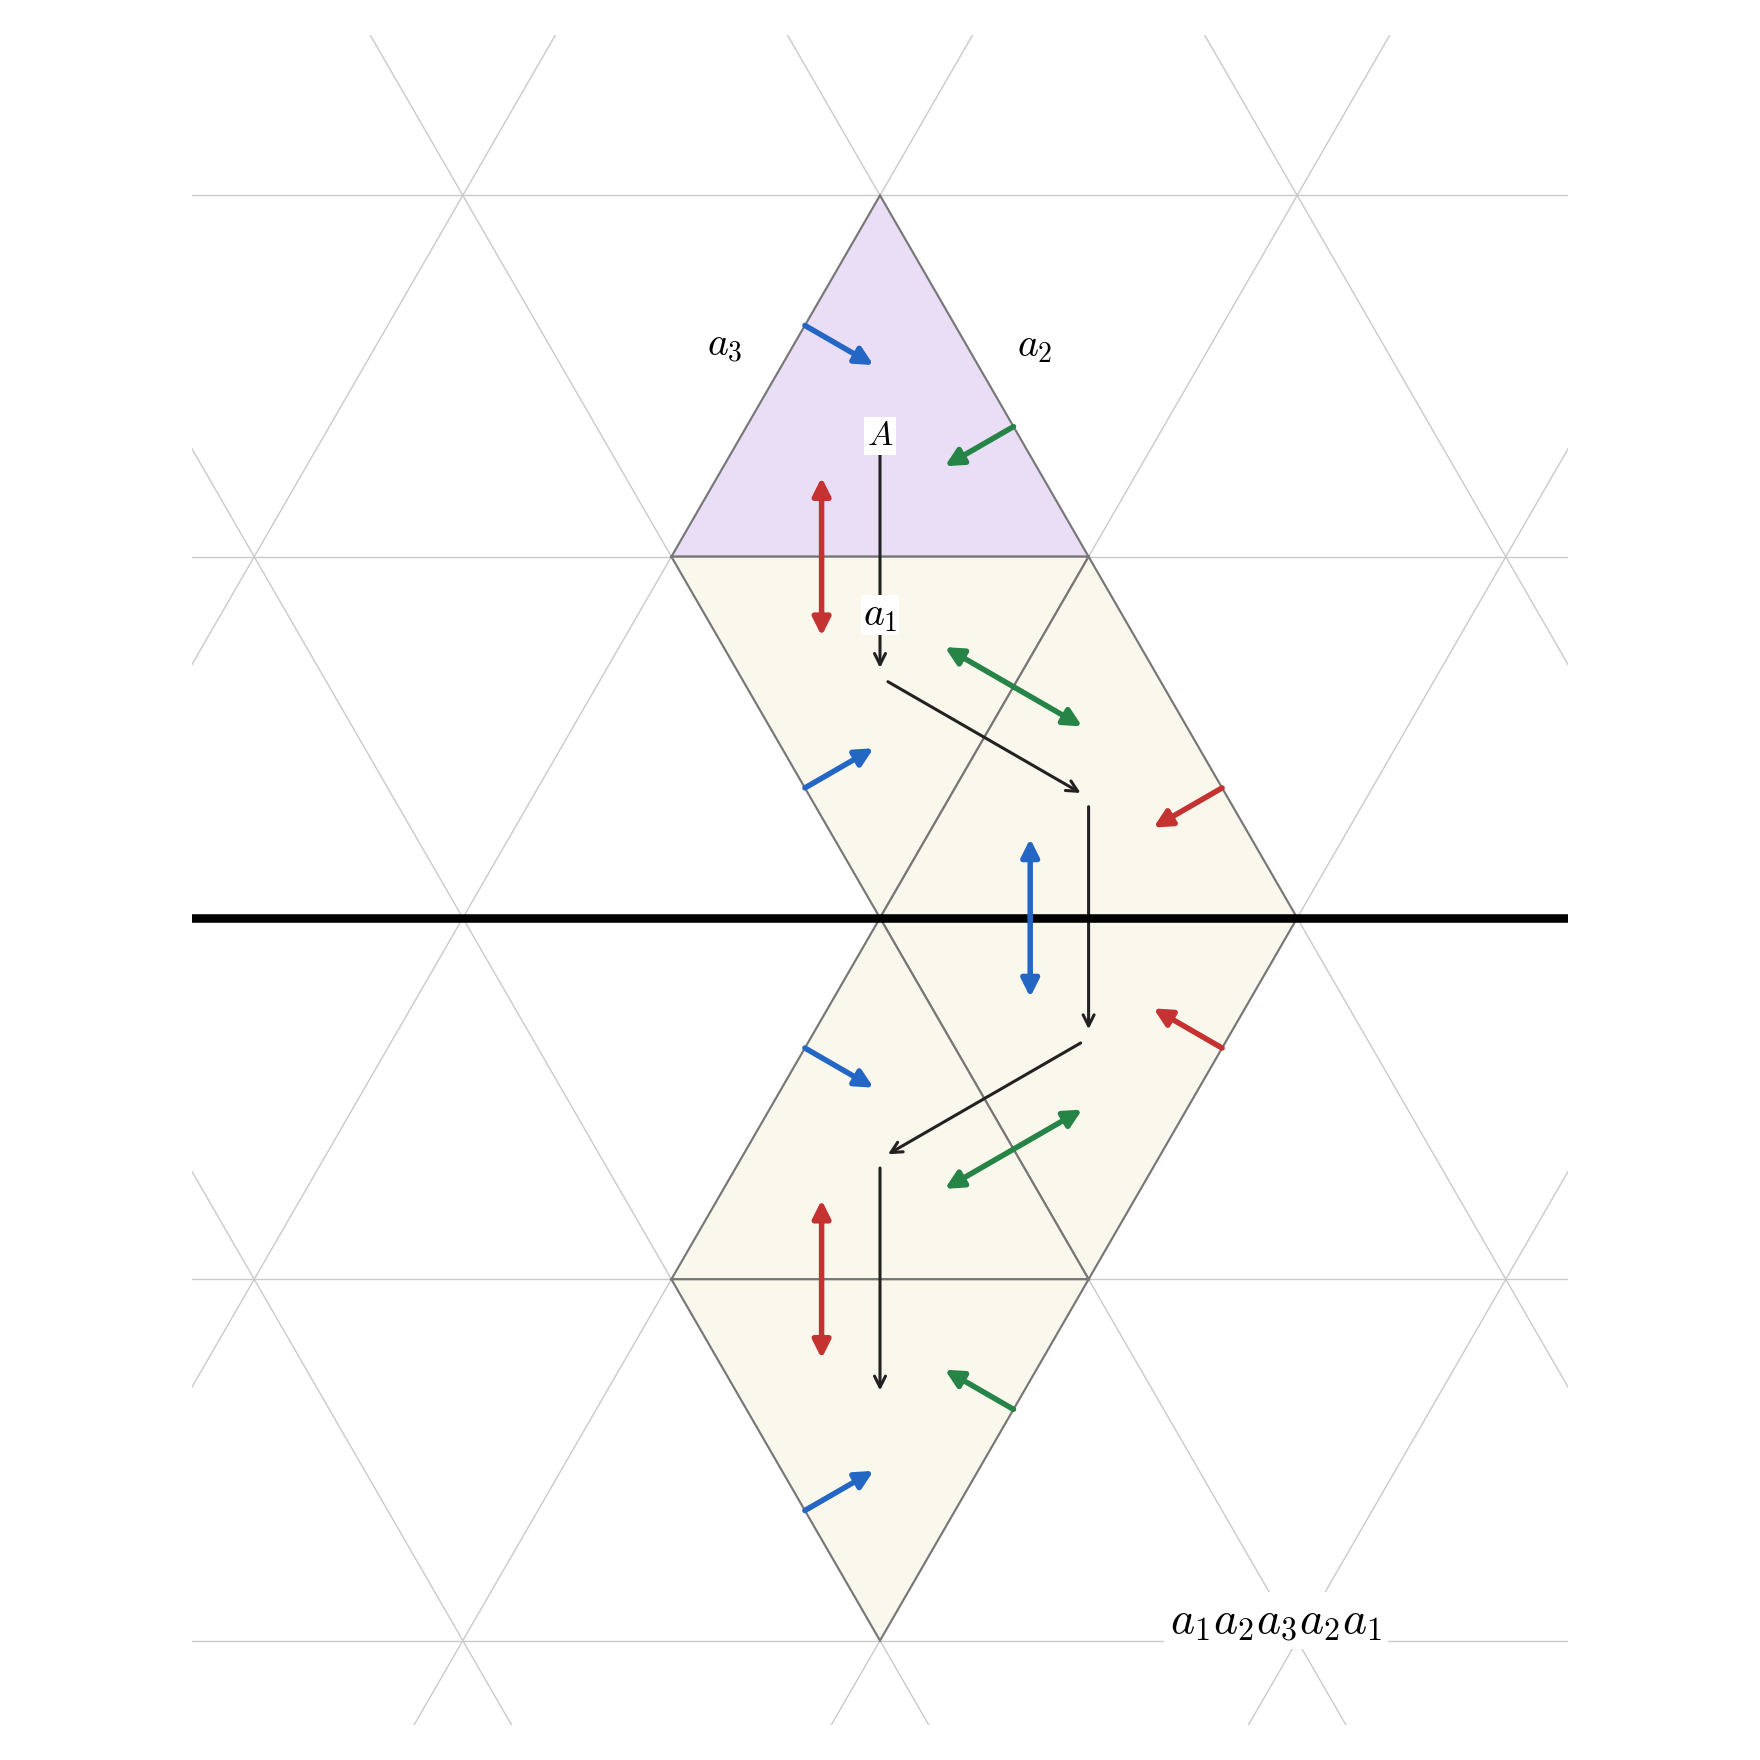
\includegraphics[width=0.60\linewidth]{affine_a2_path_12321_roots.png}
        \caption{The gallery associated to $w^{-1} = a_1a_2a_3a_2a_1$ for $w=a_1a_2a_3a_2a_1$. Note that the markings on the alcove associated to the endpoint of this gallery are a reflected version of the initial alcove, along the hyperplane marked in bold, and both $w^{-1}(\alpha_{a_2}),w^{-1}(\alpha_{a_3})$ are therefore positive. If $w = a_1a_2a_3a_2a_1w_0$ for non-empty $w_0$, then the reflecting hyperplane will still dominate some minimal root in the fundamental alcove, and the conclusion will remain the same.}
        \label{fig:Dominatingreflection}
    \end{figure}
    \par Now to complete the proof let us assume there are no indices such that $s_i=s_{i+2}$. Then $w=(s_1s_2s_3)^jw_0$ where $w_0 = \textup{[empty]}, s_1, s_1s_2$. There are no braid relations in this word, and so its Reverse ShortLex normal form for any ordering is itself by Matsumoto's Theorem 
    \cite[Theorem 3.3.1]{BjornerBrentiCoxeter}. Taking $a_1<a_2<a_3$ and applying Lemma \ref{lem:2Weyl1Root} inductively we see that
    $$
    w^{-1}\alpha_{s_2} = \begin{cases}
        w^{-1}_0\alpha_{s_2} & 2\mid j\\
        w^{-1}_0\alpha_{s_3} & 2\nmid j
    \end{cases}.
    $$
    And so in all cases, $w^{-1}\alpha_{s_2}\neq \ominus$, which means that $\ell(s_2w) = \ell (w)+1$, giving us that it is not a left descent.
%    \par So we see in combining these with Lemma \ref{lem:PossibleDescents} the only if part of the statement.
\end{proof}
\begin{proposition}\label{prop:6LetterEnoughPrecise}
    Let $w=s_1\ldots s_k$ be a word in ShortLex normal form with respect to the ordering $a_1<a_2<a_3$. Then the left descent set of $w$ is determined by the first 6 characters.
\end{proposition}
\begin{proof}
    To show this it suffices to show that the first six letters of a word in normal form determines whether it has an odd index $i$ with the property $s_i=s_{i+2}$. This follows immediately when either $s_1=s_3$ or $s_3=s_5$. So the only cases it remains to check are:
    \begin{itemize}
        \item $s_1s_2s_3s_4s_1s_4$,
        \item $s_1s_2s_3s_2s_1s_3$,
        \item $s_1s_2s_3s_1s_2s_3$.
    \end{itemize}
    where $s_i\neq s_{i+2}$ for all $i$ odd.
    \par Let us first consider $s_1s_2s_3s_4s_1s_4$. Let us suppose towards contradiction and say there exists some word $s_1s_2s_3s_4s_1s_4s_7\ldots s_k$ with odd $i\geq 7$ such that $s_{i}=s_{i+2}$. Then we see recursively by Lemma \ref{lem:abaGeneralCase} that
    $$
    s_1s_2s_3s_4s_1s_4s_7\ldots s_k \sim s_1s_2s_3s_4s_1s_4s_1\ldots
    $$
    which violates the minimality of $s_1s_2s_3s_4s_1s_4s_7\ldots s_k$ as $s_4s_1s_4s_1=s_1s_4$. So no such odd index can exist. We argue similarly for the cases $s_1s_2s_3s_2s_1s_3$. 
    \par Finally in the case $s_1s_2s_3s_1s_2s_3$, we likewise see that any $s_1s_2s_3s_1s_2s_3s_7\ldots s_k$ with odd $i\geq 7$ such that $s_{i}=s_{i+2}$ propagates back via the braid relations to a violation of lexicographic minimality.
\end{proof}

\section{Masking experiments}
To test whether the information contained in the first few tokens is sufficient for predicting the left descent set of a word of length \(\leq 36\), we ran two token-masking experiments on the ShortLex data set: one in which we masked the first \(5\) tokens, and one in which we masked all but the first \(5\). Consistent with the attention pattern in Figure \ref{fig:LeftDescents}, performance dropped substantially when the first \(5\) tokens were masked, while remaining nearly unchanged when only the first \(5\) tokens were retained. See Figure \ref{fig:MaskingAccuracy}.

\begin{figure}[h]
    \centering
    \begin{subfigure}{195 pt}
    \centering
    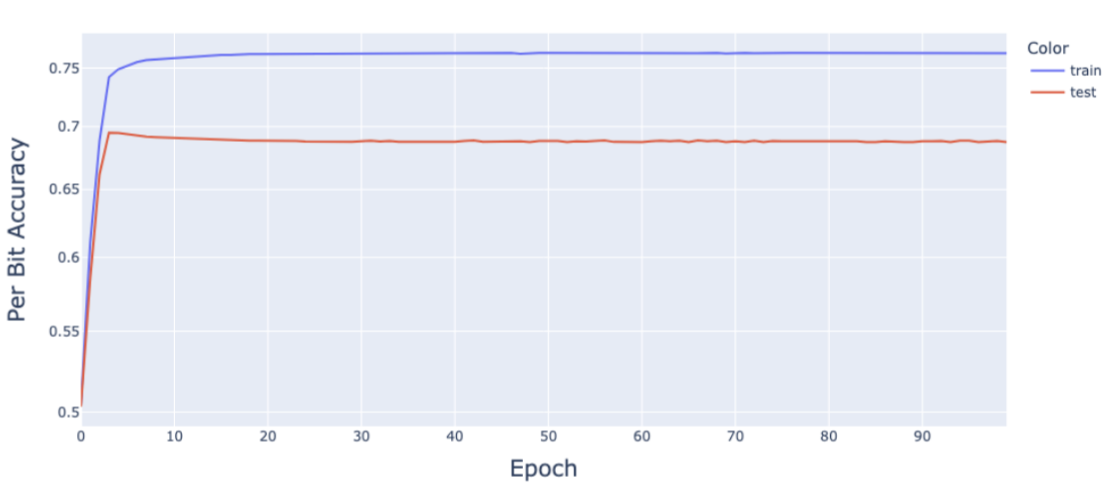
\includegraphics[width=\linewidth]{MaskFirst5.png}
    \caption{First $5$ tokens masked}  \label{fig:First5MaskedAccuracy}    
    \end{subfigure} \hfill
    \begin{subfigure}{195 pt}
    \centering    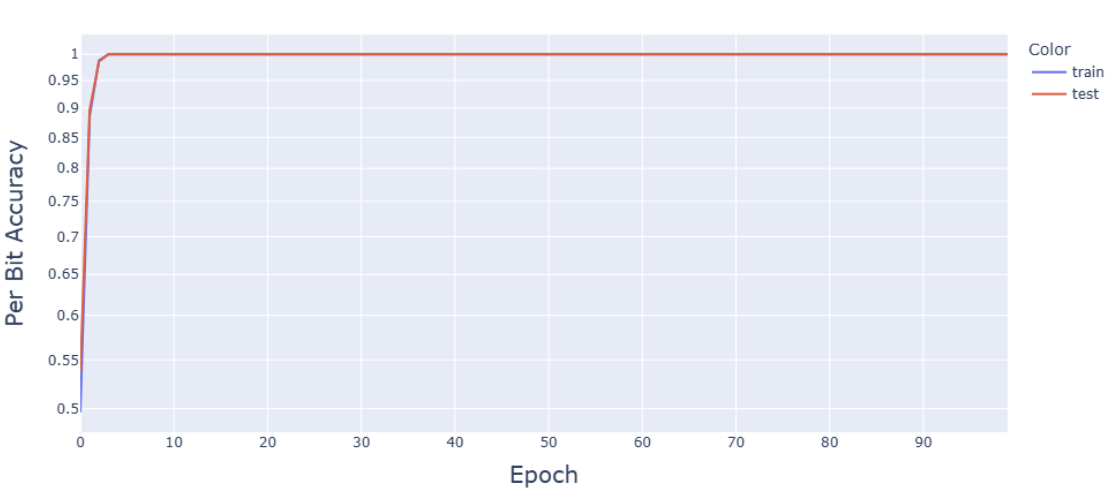
\includegraphics[width=\linewidth]{MaskAfterFirst5.png}
    \caption{All but first $5$ tokens masked}  \label{fig:AllButFirst5MaskedAccuracy}
\end{subfigure}
\caption{Model accuracy for the left descent task on ShortLex words in $\widetilde{A}_2$ when a subset of input tokens is masked during training. Test and train accuracy were nearly $100\%$ on the left descent task when no tokens were masked, stayed at nearly $100\%$ when all but the first $5$ tokens were masked, and dropped to below $70\%$ on the test set when the first $5$ tokens were masked.}
\label{fig:MaskingAccuracy}
\end{figure}


\section{Model training details and attention pattern consistency}
\emph{Model and training.} We used the TransformerLens \texttt{HookedTransformer}: $1$ layer, $d_{\mathrm{model}}=256$, $4$ heads of dimension $64$, MLP width $1024$ with ReLU, no layer normalization, learned absolute positional embeddings, causal attention, vocabulary of $3$ generators plus padding, and $3$ sigmoid outputs. All biases were frozen at zero for interpretability. There are $799{,}747$ parameters in total. Optimizer: AdamW, learning rate $10^{-4}$ (constant), $\beta=(0.9,0.98)$, weight decay $0.5$, full batch, masked binary cross-entropy. Epochs: $10{,}000$ (left) and $25{,}000$ (right). Seeds: split seed $0$, initialization seed $999$, and training seed $598$ for the published runs. Replicates $s=1,2,3$ use split seed $s$ and initialization and training seeds offset by $s$. 

\emph{Consistency of the attention patterns over multiple runs}. Test exact-set accuracy over the four runs for the ShortLex data set is $1.0000\pm0.0000$ (left descent task) and $0.9996\pm0.0004$ (right descent task), with train accuracy $1.0000$ throughout. The left descent attention concentration on the first six tokens recurred with every seed ($44$--$51\%$ of final-token attention on keys $1$--$6$, vs.\ $17\%$ uniform). The right descent effect (same parity keys matter most) also recurred in every seed. 



\section{Random and reduced word experiments}

The work reported in the main body of the paper came out of training on labeled data sets of words in ShortLex normal form in the Coxeter group $\widetilde{A}_2$. We also trained the same transformer model on the less-structured data sets of random and reduced words, where random words have letters sampled uniformly from $\{a_1, a_2, a_3\},$ while reduced words are sampled uniformly as above and then {\em reduced} by eliminating all (redundant) substrings of the form $a_ia_i$. We trained on datasets of $2000$ words at lengths $10$ and $16$. Figures \ref{fig:LeftRandomAccuracy} and \ref{fig:LeftReducedAccuracy} record the train/test accuracy of the model on the left descent task for all $4$ data sets after training has stabilized.


\begin{figure}[h]
    \centering
    \begin{subfigure}{195 pt}
    \centering
    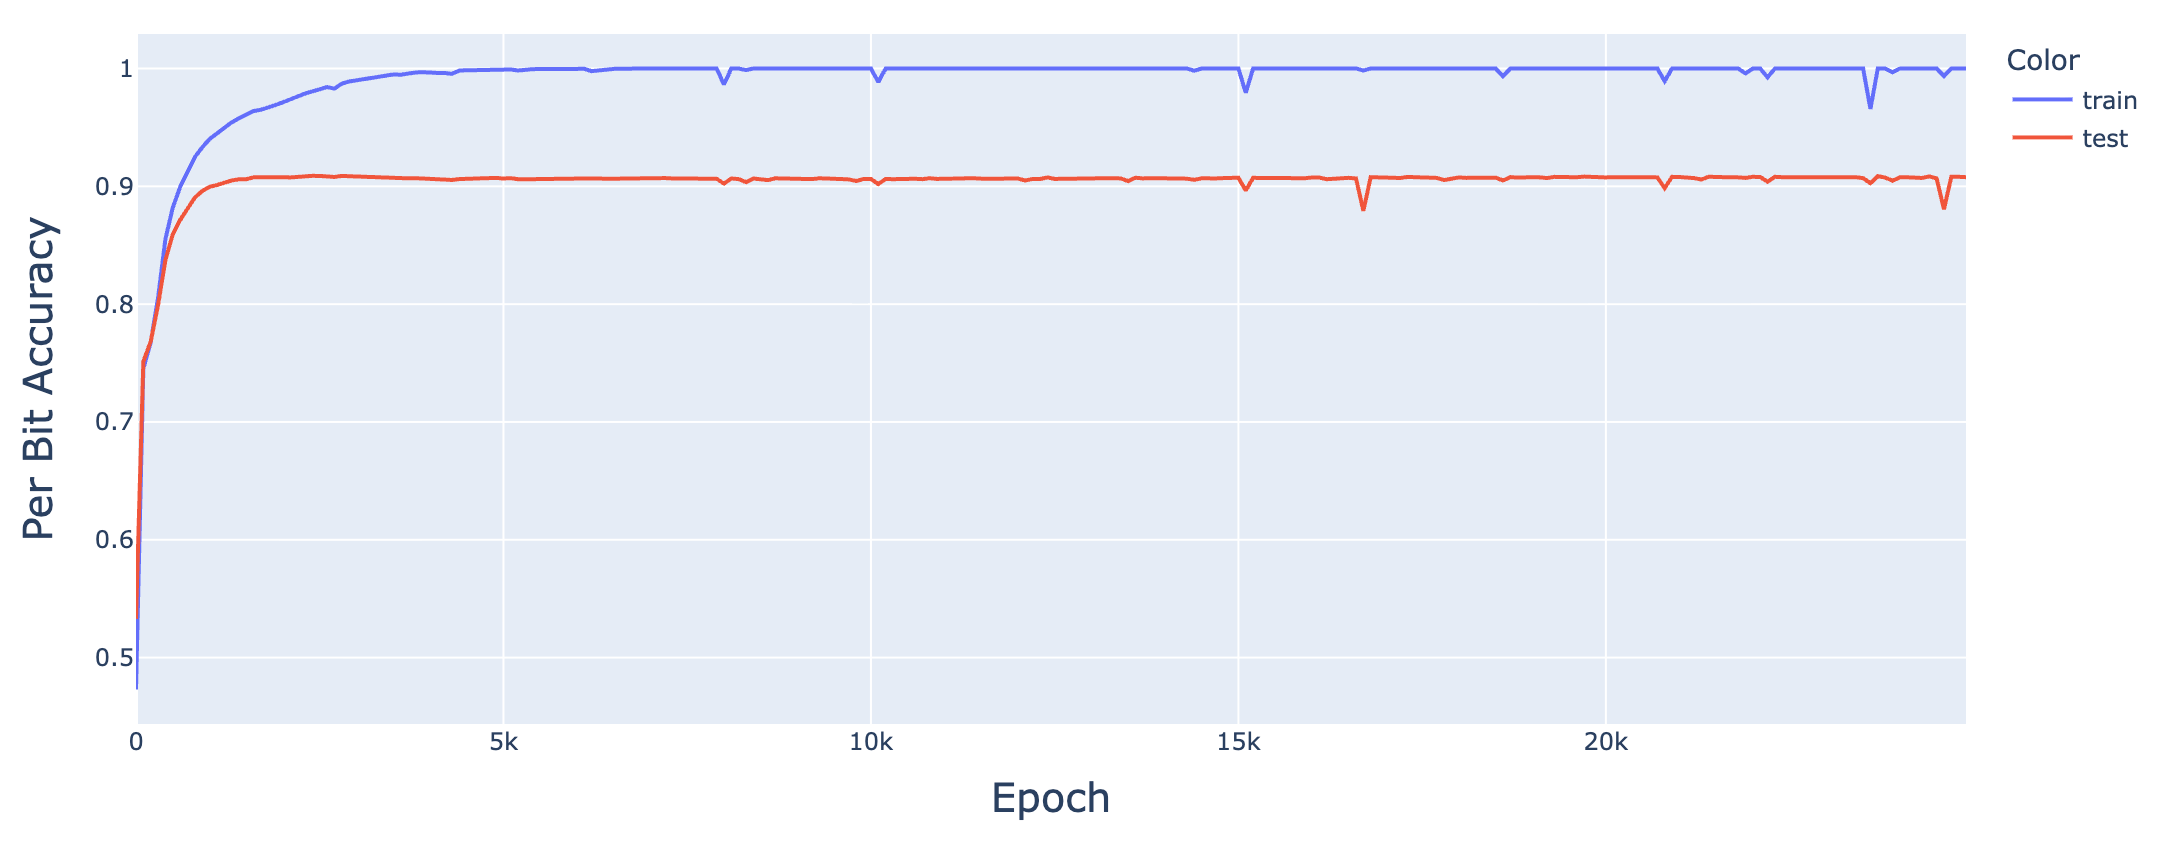
\includegraphics[width=\linewidth]{random_length_10_acc.png}
    \caption{Random words of length $10$}  \label{fig:RandomAccuracy10}    
    \end{subfigure} \hfill
    \begin{subfigure}{195 pt}
    \centering    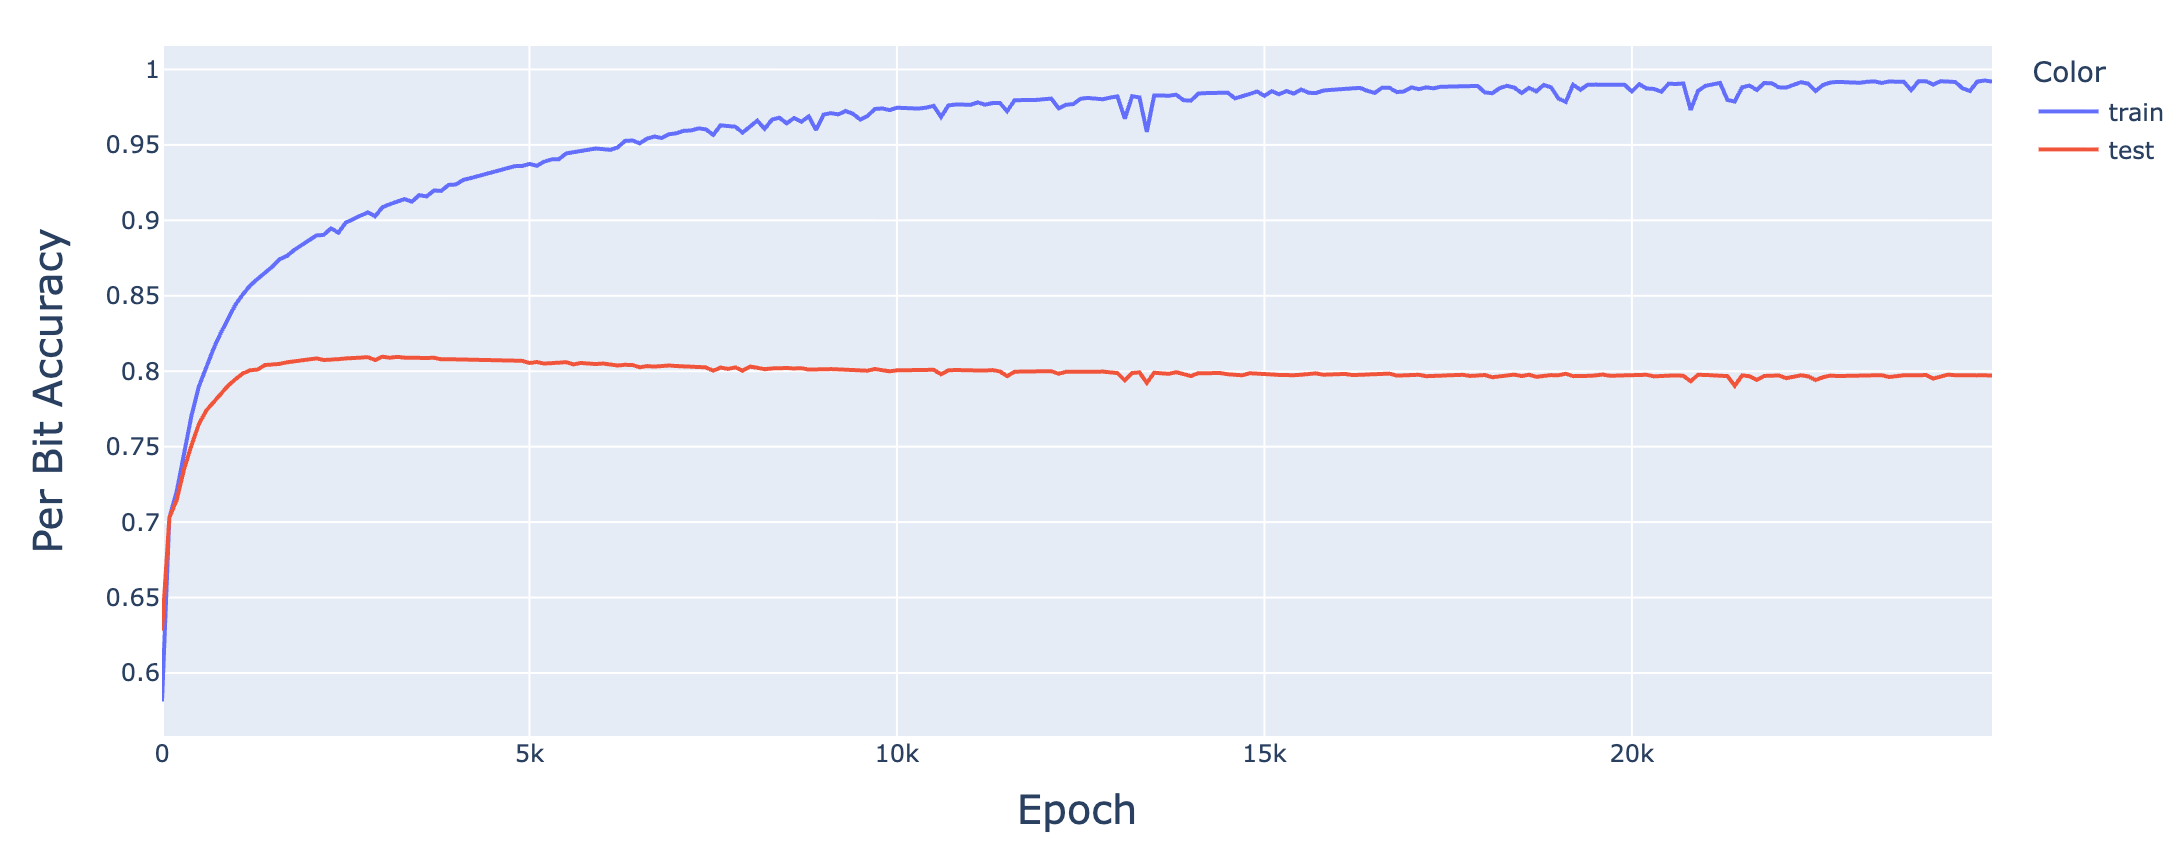
\includegraphics[width=\linewidth]{random_length_16_acc.png}
    \caption{Random words of length $16$}  \label{fig:RandomAccuracy16}
\end{subfigure}
\caption{Model accuracy for the left descent task on random words in $\widetilde{A}_2$.}
\label{fig:LeftRandomAccuracy}
\end{figure}

\begin{figure}[h]
    \centering
    \begin{subfigure}{195 pt}
    \centering
    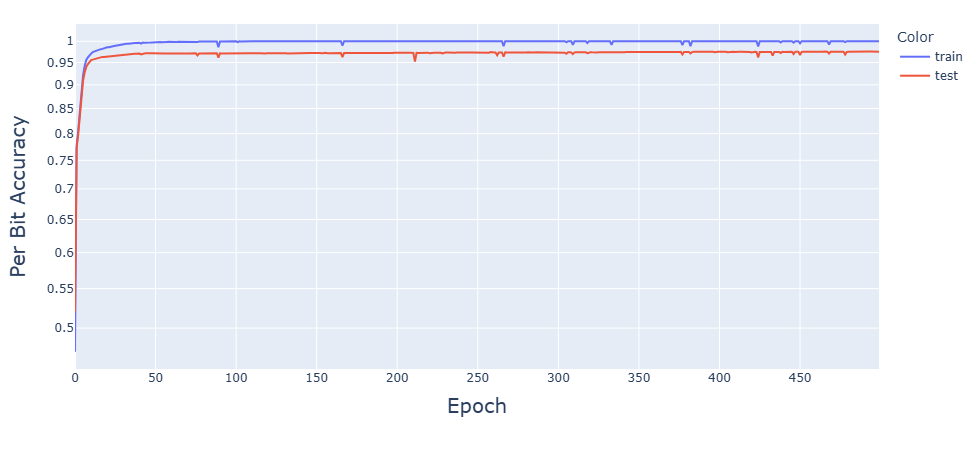
\includegraphics[width=\linewidth]{reduced_length_10_acc.png}
    \caption{Reduced words of length $10$}  \label{fig:ReducedAccuracy10}    
    \end{subfigure} \hfill
    \begin{subfigure}{195 pt}
    \centering    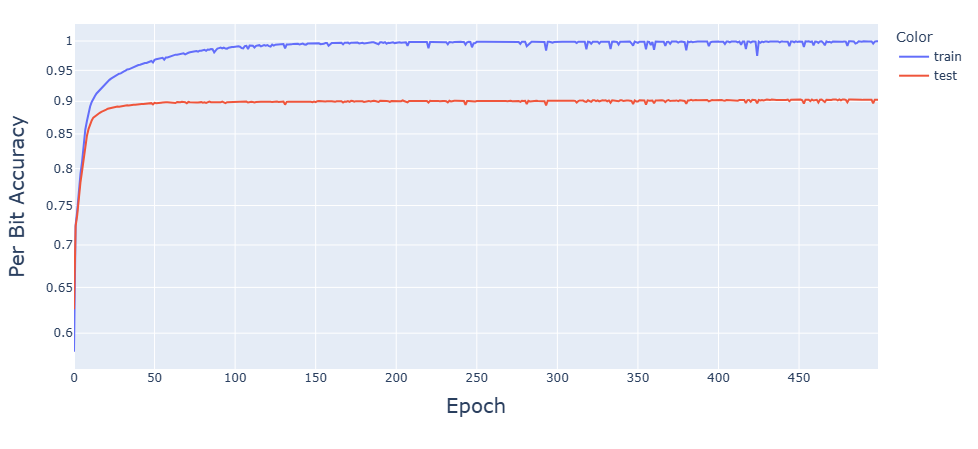
\includegraphics[width=\linewidth]{reduced_length_16_acc.png}
    \caption{Reduced words of length $16$}  \label{fig:ReducedAccuracy16}
\end{subfigure}
\caption{Model accuracy for the left descent task on reduced words in $\widetilde{A}_2$}
\label{fig:LeftReducedAccuracy}
\end{figure}

Figures \ref{fig:MiscassificationRandom} and \ref{fig:MisclassificationReduced} report misclassification rate by index on the train and test sets for random and reduced words of length $10$. Observe that the misclassification rate grows rapidly with the index, suggesting that the model has not learned a length-generalizable algorithm for determining the left descent set, in contrast to the performance of the model on the ShortLex data set.

\begin{figure}[h]
    \centering
    \begin{subfigure}{190 pt}
    \centering
    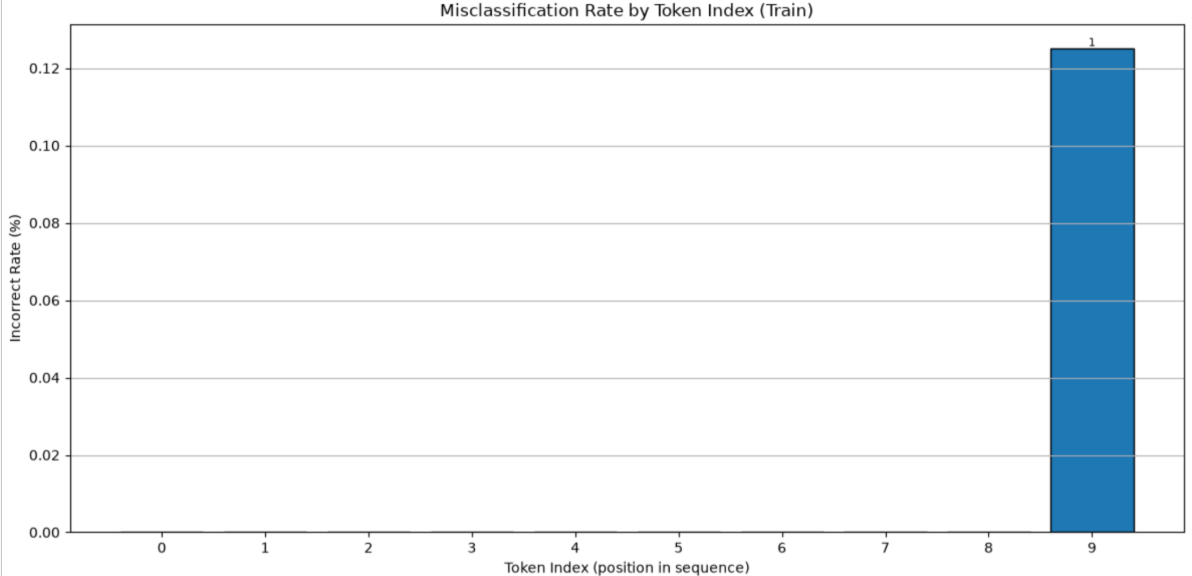
\includegraphics[width=\linewidth]{train_misclass_random.png}
    \caption{Training set misclassification by index.}  \label{fig:RandomTrainMisclass}    
    \end{subfigure} \hfill
    \begin{subfigure}{190 pt}
    \centering    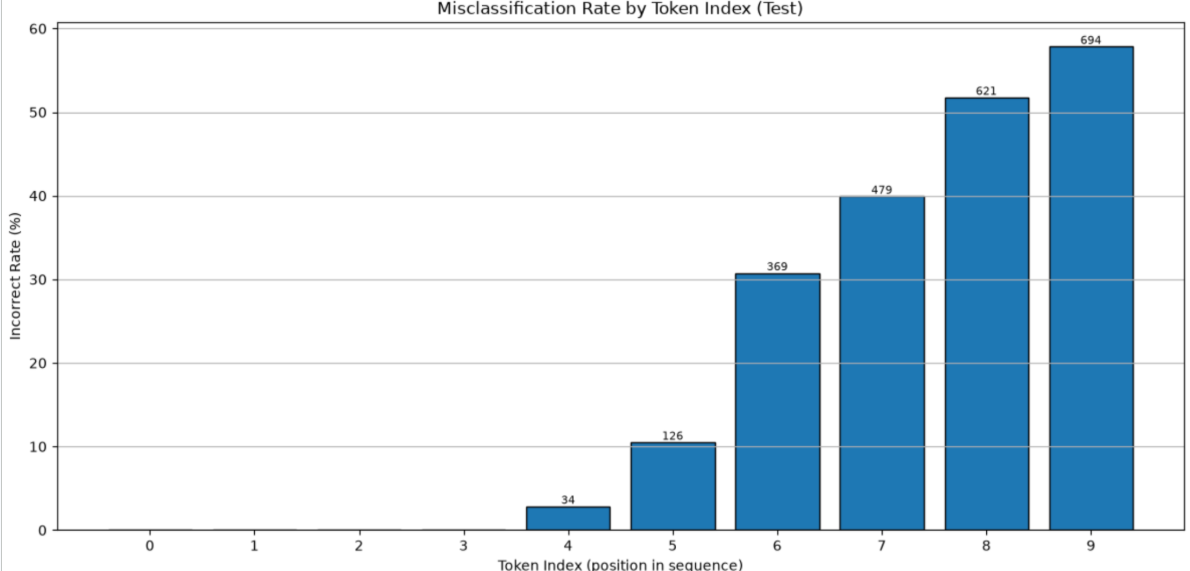
\includegraphics[width=\linewidth]{test_misclass_random.png}
    \caption{Test set misclassification by index.}  \label{fig:RandomTestMisclass}
\end{subfigure}
\caption{Misclassification rates by index for random length $10$ words in $\widetilde{A}_2$}
\label{fig:MiscassificationRandom}
\end{figure}

\begin{figure}[h]
    \centering
    \begin{subfigure}{190 pt}
    \centering
    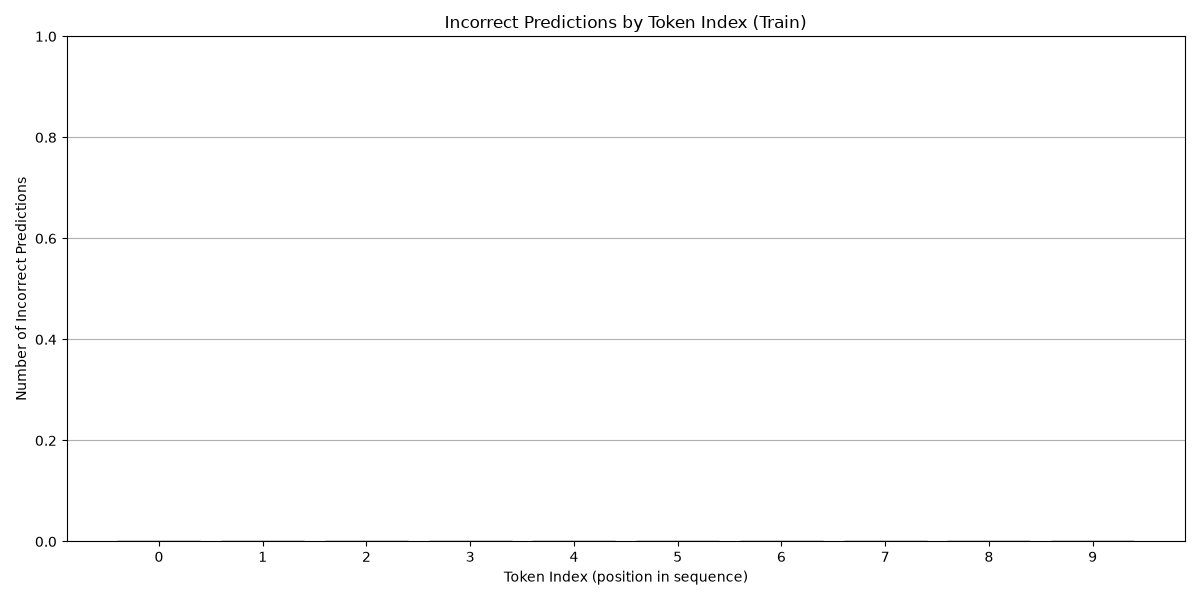
\includegraphics[width=\linewidth]{train_misclass_reduced.png}
    \caption{Train misclassifications for left descent of reduced length 10 words in $\widetilde{A}_2$.}  \label{fig:ReducedTrainMisclass}    
    \end{subfigure} \hfill
    \begin{subfigure}{190 pt}
    \centering    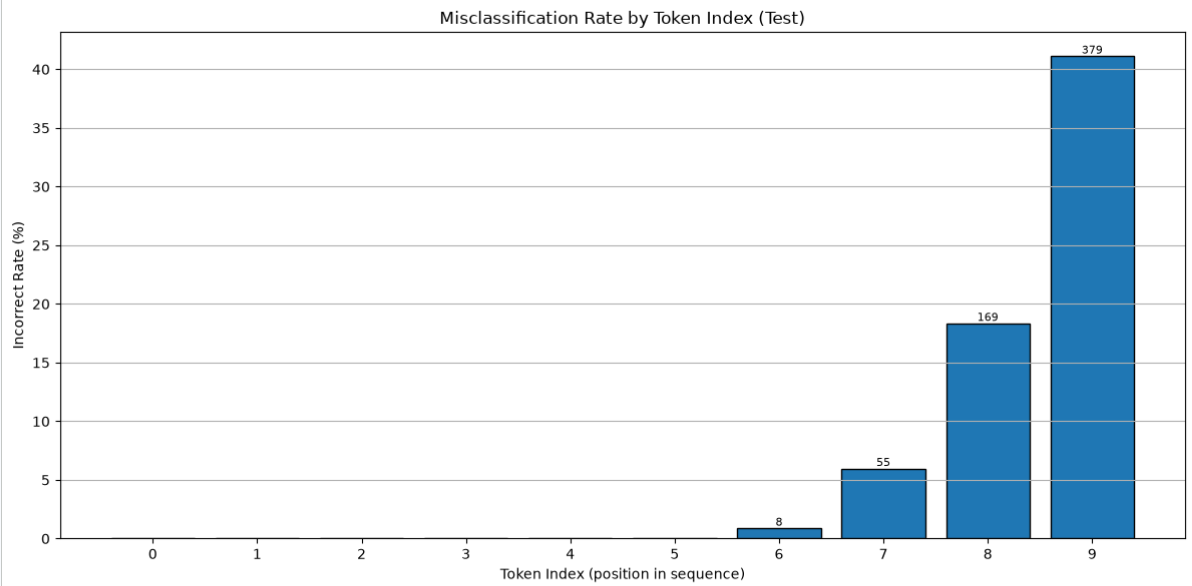
\includegraphics[width=\linewidth]{test_misclass_reduced.png}
    \caption{Test misclassifications for left descent of reduced length 10 words in $\widetilde{A}_2$.}  \label{fig:ReducedTestMisclass}
\end{subfigure}
\caption{Misclassification rates by index for reduced length $10$ words in $\widetilde{A}_2$}
\label{fig:MisclassificationReduced}
\end{figure}


\subsubsection*{Acknowledgements}
The authors are indebted to Tony Licata and Joel Gibson, who generously shared expertise and references on computation in Coxeter groups. The descent set task was Tony's idea. We gratefully acknowledge the support of the Institute for the Foundations of Machine Learning (IFML), which funded P. Ramanakrishnan's project to adapt the algorithm outlined in \citet{casselman2008computationcoxetergroupsii} to produce the data sets used to train our models. Y. Huang, A. Katyal, R. Lin, and W. Wang were supported by Boston College Undergraduate Research Fellowships to do the work on this  project during Summer 2026 through the Boston College Experimental Math and Machine Learning Lab (BCExpMMLL). This project built on a previous BCExpMMLL project with Caleb Ashley, David Ruiz De Castilla, Vanessa Rigoglioso, Roman Roy, Rob Vollbrecht, and Celina Xiong. 

\bibliographystyle{plainnat} % NeurIPS standard bibliography style
\bibliography{neurips_2026}    % Points to your references.bib file
\end{document}


\color{purple}
\section{Submission of papers to NeurIPS 2026}


Please read the instructions below carefully and follow them faithfully.


\subsection{Style}


Papers to be submitted to NeurIPS 2026 must be prepared according to the
instructions presented here. Papers may only be up to {\bf nine} pages long, including figures. \textbf{Papers that exceed the page limit will not be reviewed (or in any other way considered) for presentation at the conference.}
Additional pages \emph{containing acknowledgments, references, checklist, and optional technical appendices} do not count as content pages. 


The margins in 2026 are the same as those in previous years.


Authors are required to use the NeurIPS \LaTeX{} style files obtainable at the NeurIPS website as indicated below. Please make sure you use the current files and not previous versions. Tweaking the style files may be grounds for desk rejection.


\subsection{Retrieval of style files}


The style files for NeurIPS and other conference information are available on the website at
\begin{center}
  \url{https://neurips.cc}.
\end{center}
% The file \verb+neurips_2026.pdf+ contains these instructions and illustrates the various formatting requirements your NeurIPS paper must satisfy.


The only supported style file for NeurIPS 2026 is \verb+neurips_2026.sty+, rewritten for \LaTeXe{}. \textbf{Previous style files for \LaTeX{} 2.09,  Microsoft Word, and RTF are no longer supported.}


The \LaTeX{} style file contains three optional arguments: 
\begin{itemize}
\item \verb+final+, which creates a camera-ready copy, 
\item \verb+preprint+, which creates a preprint for submission to, e.g., arXiv, \item \verb+nonatbib+, which will not load the \verb+natbib+ package for you in case of package clash.
\end{itemize}


\paragraph{Preprint option}
If you wish to post a preprint of your work online, e.g., on arXiv, using the NeurIPS style, please use the \verb+preprint+ option. This will create a nonanonymized version of your work with the text ``Preprint. Work in progress.'' in the footer. This version may be distributed as you see fit, as long as you do not say which conference it was submitted to. Please \textbf{do not} use the \verb+final+ option, which should \textbf{only} be used for papers accepted to NeurIPS.


At submission time, please omit the \verb+final+ and \verb+preprint+ options. This will anonymize your submission and add line numbers to aid review. Please do \emph{not} refer to these line numbers in your paper as they will be removed during generation of camera-ready copies.


The file \verb+neurips_2026.tex+ may be used as a ``shell'' for writing your paper. All you have to do is replace the author, title, abstract, and text of the paper with your own.


The formatting instructions contained in these style files are summarized in Sections \ref{gen_inst}, \ref{headings}, and \ref{others} below.


\section{General formatting instructions}
\label{gen_inst}


The text must be confined within a rectangle 5.5~inches (33~picas) wide and
9~inches (54~picas) long. The left margin is 1.5~inch (9~picas).  Use 10~point
type with a vertical spacing (leading) of 11~points.  Times New Roman is the
preferred typeface throughout, and will be selected for you by default.
Paragraphs are separated by \nicefrac{1}{2}~line space (5.5 points), with no
indentation.


The paper title should be 17~point, initial caps/lower case, bold, centered
between two horizontal rules. The top rule should be 4~points thick and the
bottom rule should be 1~point thick. Allow \nicefrac{1}{4}~inch space above and
below the title to rules. All pages should start at 1~inch (6~picas) from the
top of the page.


For the final version, authors' names are set in boldface, and each name is
centered above the corresponding address. The lead author's name is to be listed
first (left-most), and the co-authors' names (if different address) are set to
follow. If there is only one co-author, list both author and co-author side by
side.


Please pay special attention to the instructions in Section \ref{others}
regarding figures, tables, acknowledgments, and references.

\section{Headings: first level}
\label{headings}


All headings should be lower case (except for first word and proper nouns),
flush left, and bold.


First-level headings should be in 12-point type.


\subsection{Headings: second level}


Second-level headings should be in 10-point type.


\subsubsection{Headings: third level}


Third-level headings should be in 10-point type.


\paragraph{Paragraphs}


There is also a \verb+\paragraph+ command available, which sets the heading in
bold, flush left, and inline with the text, with the heading followed by 1\,em
of space.


\section{Citations, figures, tables, references}
\label{others}


These instructions apply to everyone.


\subsection{Citations within the text}


The \verb+natbib+ package will be loaded for you by default.  Citations may be
author/year or numeric, as long as you maintain internal consistency.  As to the
format of the references themselves, any style is acceptable as long as it is
used consistently.


The documentation for \verb+natbib+ may be found at
\begin{center}
  \url{http://mirrors.ctan.org/macros/latex/contrib/natbib/natnotes.pdf}
\end{center}
Of note is the command \verb+\citet+, which produces citations appropriate for
use in inline text.  For example,
\begin{verbatim}
   \citet{hasselmo} investigated\dots
\end{verbatim}
produces
\begin{quote}
  Hasselmo, et al.\ (1995) investigated\dots
\end{quote}


If you wish to load the \verb+natbib+ package with options, you may add the
following before loading the \verb+neurips_2026+ package:
\begin{verbatim}
   \PassOptionsToPackage{options}{natbib}
\end{verbatim}


If \verb+natbib+ clashes with another package you load, you can add the optional
argument \verb+nonatbib+ when loading the style file:
\begin{verbatim}
   \usepackage[nonatbib]{neurips_2026}
\end{verbatim}


As submission is double blind, refer to your own published work in the third
person. That is, use ``In the previous work of Jones et al.\ [4],'' not ``In our
previous work [4].'' If you cite your other papers that are not widely available
(e.g., a journal paper under review), use anonymous author names in the
citation, e.g., an author of the form ``A.\ Anonymous'' and include a copy of the anonymized paper in the supplementary material.


\subsection{Footnotes}


Footnotes should be used sparingly.  If you do require a footnote, indicate
footnotes with a number\footnote{Sample of the first footnote.} in the
text. Place the footnotes at the bottom of the page on which they appear.
Precede the footnote with a horizontal rule of 2~inches (12~picas).


Note that footnotes are properly typeset \emph{after} punctuation
marks.\footnote{As in this example.}


\subsection{Figures}


\begin{figure}
  \centering
  \fbox{\rule[-.5cm]{0cm}{4cm} \rule[-.5cm]{4cm}{0cm}}
  \caption{Sample figure caption. Explain what the figure shows and add a key take-away message to the caption.}
\end{figure}


All artwork must be neat, clean, and legible. Lines should be dark enough for
 reproduction purposes. The figure number and caption always appear after the
figure. Place one line space before the figure caption and one line space after
the figure. The figure caption should be lower case (except for the first word and proper nouns); figures are numbered consecutively.


You may use color figures.  However, it is best for the figure captions and the
paper body to be legible if the paper is printed in either black/white or in
color.


\subsection{Tables}


All tables must be centered, neat, clean, and legible.  The table number and
title always appear before the table.  See Table~\ref{sample-table}.


Place one line space before the table title, one line space after the
table title, and one line space after the table. The table title must
be lower case (except for the first word and proper nouns); tables are
numbered consecutively.


Note that publication-quality tables \emph{do not contain vertical rules}. We
strongly suggest the use of the \verb+booktabs+ package, which allows for
typesetting high-quality, professional tables:
\begin{center}
  \url{https://www.ctan.org/pkg/booktabs}
\end{center}
This package was used to typeset Table~\ref{sample-table}.


\begin{table}
  \caption{Sample table caption. Explain what the table shows and add a key take-away message to the caption.}
  \label{sample-table}
  \centering
  \begin{tabular}{lll}
    \toprule
    \multicolumn{2}{c}{Part}                   \\
    \cmidrule(r){1-2}
    Name     & Description     & Size ($\mu$m) \\
    \midrule
    Dendrite & Input terminal  & $\approx$100     \\
    Axon     & Output terminal & $\approx$10      \\
    Soma     & Cell body       & up to $10^6$  \\
    \bottomrule
  \end{tabular}
\end{table}

\subsection{Math}
Note that display math in bare TeX commands will not create correct line numbers for submission. Please use LaTeX (or AMSTeX) commands for unnumbered display math. (You really shouldn't be using \$\$ anyway; see \url{https://tex.stackexchange.com/questions/503/why-is-preferable-to} and \url{https://tex.stackexchange.com/questions/40492/what-are-the-differences-between-align-equation-and-displaymath} for more information.)

\subsection{Final instructions}

Do not change any aspects of the formatting parameters in the style files.  In
particular, do not modify the width or length of the rectangle the text should
fit into, and do not change font sizes. Please note that pages should be
numbered.


\section{Preparing PDF files}


Please prepare submission files with paper size ``US Letter,'' and not, for
example, ``A4.''


Fonts were the main cause of problems in the past years. Your PDF file must only
contain Type 1 or Embedded TrueType fonts. Here are a few instructions to
achieve this.


\begin{itemize}


\item You should directly generate PDF files using \verb+pdflatex+.


\item You can check which fonts a PDF files uses.  In Acrobat Reader, select the
  menu Files$>$Document Properties$>$Fonts and select Show All Fonts. You can
  also use the program \verb+pdffonts+ which comes with \verb+xpdf+ and is
  available out-of-the-box on most Linux machines.


\item \verb+xfig+ ``patterned'' shapes are implemented with bitmap fonts.  Use
  "solid" shapes instead.


\item The \verb+\bbold+ package almost always uses bitmap fonts.  You should use
  the equivalent AMS Fonts:
\begin{verbatim}
   \usepackage{amsfonts}
\end{verbatim}
followed by, e.g., \verb+\mathbb{R}+, \verb+\mathbb{N}+, or \verb+\mathbb{C}+
for $\mathbb{R}$, $\mathbb{N}$ or $\mathbb{C}$.  You can also use the following
workaround for reals, natural and complex:
\begin{verbatim}
   \newcommand{\RR}{I\!\!R} %real numbers
   \newcommand{\Nat}{I\!\!N} %natural numbers
   \newcommand{\CC}{I\!\!\!\!C} %complex numbers
\end{verbatim}
Note that \verb+amsfonts+ is automatically loaded by the \verb+amssymb+ package.


\end{itemize}


If your file contains type 3 fonts or non embedded TrueType fonts, we will ask
you to fix it.


\subsection{Margins in \LaTeX{}}


Most of the margin problems come from figures positioned by hand using
\verb+\special+ or other commands. We suggest using the command
\verb+\includegraphics+ from the \verb+graphicx+ package. Always specify the
figure width as a multiple of the line width as in the example below:
\begin{verbatim}
   \usepackage[pdftex]{graphicx} ...
   \includegraphics[width=0.8\linewidth]{myfile.pdf}
\end{verbatim}
See Section 4.4 in the graphics bundle documentation
(\url{http://mirrors.ctan.org/macros/latex/required/graphics/grfguide.pdf})


A number of width problems arise when \LaTeX{} cannot properly hyphenate a
line. Please give LaTeX hyphenation hints using the \verb+\-+ command when
necessary.

\begin{ack}
Use unnumbered first level headings for the acknowledgments. All acknowledgments
go at the end of the paper before the list of references. Moreover, you are required to declare
funding (financial activities supporting the submitted work) and competing interests (related financial activities outside the submitted work).
More information about this disclosure can be found at: \url{https://neurips.cc/Conferences/2026/PaperInformation/FundingDisclosure}.


Do {\bf not} include this section in the anonymized submission, only in the final paper. You can use the \texttt{ack} environment provided in the style file to automatically hide this section in the anonymized submission.
\end{ack}

\section*{References}


References follow the acknowledgments in the camera-ready paper. Use unnumbered first-level heading for
the references. Any choice of citation style is acceptable as long as you are
consistent. It is permissible to reduce the font size to \verb+small+ (9 point)
when listing the references.
Note that the Reference section does not count towards the page limit.
\medskip


{
\small


[1] Alexander, J.A.\ \& Mozer, M.C.\ (1995) Template-based algorithms for
connectionist rule extraction. In G.\ Tesauro, D.S.\ Touretzky and T.K.\ Leen
(eds.), {\it Advances in Neural Information Processing Systems 7},
pp.\ 609--616. Cambridge, MA: MIT Press.


[2] Bower, J.M.\ \& Beeman, D.\ (1995) {\it The Book of GENESIS: Exploring
  Realistic Neural Models with the GEneral NEural SImulation System.}  New York:
TELOS/Springer--Verlag.


[3] Hasselmo, M.E., Schnell, E.\ \& Barkai, E.\ (1995) Dynamics of learning and
recall at excitatory recurrent synapses and cholinergic modulation in rat
hippocampal region CA3. {\it Journal of Neuroscience} {\bf 15}(7):5249-5262.
}


%%%%%%%%%%%%%%%%%%%%%%%%%%%%%%%%%%%%%%%%%%%%%%%%%%%%%%%%%%%%

\appendix

\section{Technical appendices and supplementary material}
Technical appendices with additional results, figures, graphs, and proofs may be submitted with the paper submission before the full submission deadline (see above). You can upload a ZIP file for videos or code, but do not upload a separate PDF file for the appendix. There is no page limit for the technical appendices. 

Note: Think of the appendix as ``optional reading'' for reviewers. The paper must be able to stand alone without the appendix; for example, adding critical experiments that support the main claims to an appendix is inappropriate. 


\bibliographystyle{plainnat} % NeurIPS standard bibliography style
\bibliography{neurips_2026}    % Points to your references.bib file
\end{document}